\documentclass[]{scrartcl}
% Лицензия
% Apache License Version 2.0, January 2004
% http://www.apache.org/licenses/
% Copyright [2020] [Kirill A. Murashev]
% Licensed under the Apache License, Version 2.0 (the "License"); you may not use this file except in compliance with the License. You may obtain a copy of the License at
% http://www.apache.org/licenses/LICENSE-2.0
% Unless required by applicable law or agreed to in writing, software
% distributed under the License is distributed on an "AS IS" BASIS,
% WITHOUT WARRANTIES OR CONDITIONS OF ANY KIND, either express or implied.
% See the License for the specific language governing permissions and limitations under the License.


%%% Работа с русским языком
\usepackage{cmap}					% поиск в PDF
\usepackage{mathtext} 				% русские буквы в формулах
\usepackage{fontspec}
\defaultfontfeatures{Renderer=Basic,Ligatures={TeX}}
\setmainfont{CMU Serif}
\setsansfont{CMU Sans Serif}
\setmonofont{CMU Typewriter Text}
\usepackage[english,russian]{babel}
%\usepackage[T1,T2A]{fontenc}			% кодировка
%\usepackage[lutf8]{luainputenc}			% кодировка исходного текста
%\usepackage[english,russian]{babel}	% локализация и переносы
\usepackage{indentfirst}            % красная строка
\usepackage{misccorr}               % доработки для babel
\frenchspacing                      % французский стиль пробелов

%\usepackage{beton} %изменение шрифта для тёмной цветовой схемы
%\usepackage{concrete}
%%% Дополнительная работа с математикой
\usepackage{amsmath,amsfonts,amssymb,amsthm,mathtools} % AMS
\usepackage{icomma} % "Умная" запятая: $0,2$ --- число, $0, 2$ --- перечисление

%% Номера формул
%\mathtoolsset{showonlyrefs=true} % Показывать номера только у тех формул, на которые есть \eqref{} в тексте.
%\usepackage{leqno} % Нумерация формул слева

%% Перенос знаков в формулах (по Львовскому)
\newcommand*{\hm}[1]{#1\nobreak\discretionary{}
	{\hbox{$\mathsurround=0pt #1$}}{}}

%%% Работа с картинками
\usepackage{graphicx}  % Для вставки рисунков
\graphicspath{{Images/}}  % папки с картинками
\setlength\fboxsep{3pt} % Отступ рамки \fbox{} от рисунка
\setlength\fboxrule{1pt} % Толщина линий рамки \fbox{}
\usepackage{wrapfig} % Обтекание рисунков текстом

%%% Работа с таблицами
\usepackage{array, tabularx, tabulary, booktabs, xtab} % Дополнительная работа с таблицами
\usepackage{longtable}  % Длинные таблицы
\usepackage{multirow} % Слияние строк в таблице

%%% Теоремы
\theoremstyle{plain} % Это стиль по умолчанию, его можно не переопределять.
\newtheorem{theorem}{Теорема}[section]
\newtheorem{proposition}[theorem]{Утверждение}

\theoremstyle{definition} % "Определение"
\newtheorem{corollary}{Следствие}[theorem]
\newtheorem{problem}{Задача}[section]

\theoremstyle{remark} % "Примечание"
\newtheorem*{nonum}{Решение}

%%% Программирование
\usepackage{etoolbox} % логические операторы

\usepackage{lastpage} % Узнать, сколько всего страниц в документе.

\usepackage{keyval}

\usepackage{totcount} % Узнать, сколько всего объектов в документе.

%\usepackage{xcolor-solarized}

%%% Страница
%\usepackage{extsizes} % Возможность сделать 14-й шрифт
%\usepackage{geometry} % Простой способ задавать поля
%	\geometry{top=25mm}
%	\geometry{bottom=35mm}
%	\geometry{left=35mm}
%	\geometry{right=20mm}
%

%\usepackage{fancyhdr} % Колонтитулы

%	\pagestyle{fancy}
%\renewcommand{\headrulewidth}{0pt}  % Толщина линейки, отчеркивающей верхний колонтитул
%\fancyhf{}
%\lhead{Часть \thepart}
%\chead{Глава \thechapter}
%\rhead{Раздел \thesection}
%\lfoot{version 0.251}
%\cfoot{\today} % По умолчанию здесь номер страницы
%\rfoot{\thepage/\ref{LastPage}}
%\pagestyle{fancy}

%\usepackage{setspace} % Интерлиньяж
%\onehalfspacing % Интерлиньяж 1.5
%\doublespacing % Интерлиньяж 2
%\singlespacing % Интерлиньяж 1

\usepackage{soul} % Модификаторы начертания

\usepackage[usenames,dvipsnames,svgnames,table,rgb]{xcolor} % Подключение пакета для задания цвета

%\definecolor{Backcolor}{HTML}{042029} % Задание цвета для фона
%\definecolor{Textcolor}{HTML}{819090} % Задание цвета для текста
%\pagecolor{Backcolor}                 % Подключение тёмной
%\color{Textcolor}                     % темы

\usepackage{csquotes} % Ещё инструменты для ссылок

\usepackage[backend=biber,bibencoding=utf8,sorting=ynt,maxcitenames=5,sortupper=true,date=iso]{biblatex} % подключение пакета для работы с автоматизированной библиографией

%\usepackage[style=authoryear,maxcitenames=2,backend=biber,sorting=nty]{biblatex}

%\renewcommand\bibname{Источники информации} % Переопределение названия для библиографии

\usepackage{multicol} % Несколько колонок

\usepackage{microtype}              %<-- added for better inter word spacing

\usepackage{tabularx}

\usepackage{tikz} % Работа с графикой
\usepackage{pgfplots}
\usepackage{pgfplotstable}

\usepackage{eqlist}

\usepackage{desclist} % Дополнительное окружение для списка Глоссария

\usepackage{lineno} % Нумерация строк

\setcounter{tocdepth}{8} % Глубина оглавления

% подавление висячих строк
\clubpenalty=400 % Разрешение = 300, абсолютный запрет = 10000
\widowpenalty=400 % Увеличиваем эти числа до тех пор, пока не начнёт увеличиваться количество страниц.

% Выбор между разрежением и переполнением
\tolerance=500 % max=10000, default=200

\looseness=-1 % иногда можно удлинять страницу на одну строку.

\hfuzz=2.5pt % иногда можно вылезти за край строки на 2.5 pt.

\usepackage{calc} % Вычисления

\usepackage{scrlayer-scrpage} % Стиль страницы

\usepackage{lineno} % нумерация строк

%\pagestyle{scrpage}

%\usepackage{concrete}

\usepackage{booktabs}

\usepackage[owncaptions]{vhistory} % Log of versions

\usepackage{progressbar} % Формирование линейки, показывающей прогресс в работе

\usepackage{epigraph} % работа с эпиграфами

\usepackage {listings}
\lstloadlanguages{[Latex]Tex, bash, R, Python, SQL}
\lstset{extendedchars=true , % включаем не латиницу
frame=tb, % рамка сверху и снизу
commentstyle=\itshape , % шрифт для комментариев
stringstyle =\ttfamily % шрифт для строк
%keywordstyle=\color{blue}
}

%\usepackage{titling} %дополнительная настройка титульного листа

\setcounter{secnumdepth}{8} % Установка глубины нумерации заголовков

% Работа с гиперрсылками, подключается последним
\usepackage{hyperref}       % Подключение пакета для работы с гиперссылками
\hypersetup{				% Гиперссылки
	unicode=true,           % русские буквы в раздела PDF
	pdftitle={Искусственный интеллект в~оценке стоимости},   % Заголовок
	pdfauthor={К.\,А.~Мурашев},      % Автор
	pdfsubject={Системы поддержки принятия решений, основанные на искусственном интеллекте},      % Тема
	pdfcreator={К.\,А.~Мурашев}, % Создатель
	pdfproducer={К.\,А.~Мурашев}, % Производитель
	pdfkeywords={Искусственный интеллект, машинное обучение, математические методы, оценочная деятельность, цифровая экономика, Data Science, анализ данных} % Ключевые слова
	colorlinks=true,       	% false: ссылки в рамках; true: цветные ссылки
	linkcolor=red,          % внутренние ссылки
	citecolor=green,        % на библиографию
	filecolor=magenta,      % на файлы
	urlcolor=blue           % на URL
}

\usepackage{pgfplots} 
\pgfplotsset{compat=1.15}
\usepackage{mathrsfs}
\usetikzlibrary{arrows}
%\usepackage{url}

%\usepackage{totpages}

%\usepackage[strings]{underscore}

%\author{К.\,А.~Мурашев\thanks {\href{kirill.murashev@tutanota.de}{kirill.murashev@tutanota.de}, \href{https://t.me/Maas\_88}{https://t.me/Maas\_88}, \href{https://www.facebook.com/murashev.kirill}{https://www.facebook.com/murashev.kirill}}}
%\title{\Large Современные системы поддержки принятия решений оценщиками, основанные на~применении методов машинного обучения: практическое руководство по~применению языка программирования R в~повседневной практике оценщика}
%\date{\today}

%\normalsize

% Макрос для рисунков, обтекаемых текстом
\newcommand*{\EpsWrapD}[7]{%
	\begin{wrapfigure}[#5]{#3}{#2 \textwidth} % #3=l,r,L,R
		\begin{center} \sffamily
			\includegraphics*[width= #2 \textwidth ]{#1} % 1-имя файла и метка заодно,
			% 2-ширина рисунка (доля от ширины страницы)
			\vspace{-#7mm} % #7: сократить расстояние между подписью снизу и рисунком
			\caption{\label{fig:#1}#4} % #4 - подпись под рисунком
			\vspace{-#6pt}
		\end{center}% #6: сократить расстояние между подписью снизу и текстом после таблицы 
	\end{wrapfigure}}
%
% макрос для создания таблицы, обтекаемой текстом
\newcommand*{\TableBE}[5]{
	\begin{table}[#1] %\captionabove
		\vspace*{-#5mm}
		\centering \sffamily \caption{\label{tab:#2}#3} \begin{tabular}{#4} \toprule }
		
		\newcommand*{\TableEN}[3]{
			\bottomrule \end{tabular}
		\vspace{-#2mm} \small \begin{flushleft} #1 \end{flushleft}
		\vspace{-#3mm}
\end{table}}


\addbibresource{/home/kaarlahti/TresoritDrive/Methodics/My/AI_for_valuers/Book/AI_for_valuers_book/Basic_principles.bib}
\addbibresource{/home/kaarlahti/TresoritDrive/Methodics/My/AI_for_valuers/Book/AI_for_valuers_book/LaTeX.bib}
\addbibresource{/home/kaarlahti/TresoritDrive/Methodics/My/AI_for_valuers/Book/AI_for_valuers_book/Mathstat.bib}
\addbibresource{/home/kaarlahti/TresoritDrive/Methodics/My/AI_for_valuers/Book/AI_for_valuers_book/Murashev.bib}
\addbibresource{/home/kaarlahti/TresoritDrive/Methodics/My/AI_for_valuers/Book/AI_for_valuers_book/Python.bib}
\addbibresource{/home/kaarlahti/TresoritDrive/Methodics/My/AI_for_valuers/Book/AI_for_valuers_book/R.bib}
\addbibresource{/home/kaarlahti/TresoritDrive/Methodics/My/AI_for_valuers/Book/AI_for_valuers_book/RussianLaws.bib}
\addbibresource{/home/kaarlahti/TresoritDrive/Methodics/My/AI_for_valuers/Book/AI_for_valuers_book/Sci&Tech.bib}
\addbibresource{/home/kaarlahti/TresoritDrive/Methodics/My/AI_for_valuers/Book/AI_for_valuers_book/Valuation.bib}
\addbibresource{/home/kaarlahti/TresoritDrive/Methodics/My/AI_for_valuers/Book/AI_for_valuers_book/ValuationStandards.bib}
\addbibresource{/home/kaarlahti/TresoritDrive/Methodics/My/AI_for_valuers/Book/AI_for_valuers_book/ZHZL.bib}

\pagestyle{headings} 
\markright{Искусственный интеллект в~оценке стоимости}
\usepackage{pgfplots}
\pgfplotsset{compat=1.15}
\usepackage{mathrsfs}
\usetikzlibrary{arrows}

%\usepackage{polyglossia}

%\usepackage{minted}

\newtheorem{Thexmpl}[theorem]{Пример}

\usepackage[inkscapearea=page]{svg}
\usepackage{adjustbox}


\title{Очень краткое введение в~математическую статистику, основанную на~частотном подходе, для~оценщиков}
\author{К.\,А.\,Мурашев}

\begin{document}

\maketitle

\begin{abstract}
	Какую~бы работу не~выполнял оценщик, во~всех случаях он~имеет дело с~информацией и~данными. Часто эти~данные представляют собой числа либо могут быть формализованы иным образом. В~любом случае требуется алгоритмическая обработка входных данных и~преобразование их~в~информацию, а~в~некоторых случаях "--- в~знания. Целью данного фрагмента является формирование общих представлений об~основных понятиях и~методах математической статистики, необходимых современному оценщику. Автор постарался прибегать к~минимальному числу формул и~сложных определений, хотя это~и~не~вполне получилось. Поскольку конечной целью всей работы является цифровизация оценочной деятельности, в~тексте приводятся короткие листинги на~языках R и~Python, позволяющие реализовать то, о~чём говорится в~тексте. В~данном фрагменте рассматривается \href{https://ru.wikipedia.org/wiki/Частотная_вероятность}{частотный подход} к~вероятности~\cite{Wiki:Freq-probability}. Вопросы  \href{https://ru.wikipedia.org/wiki/Байесовская_вероятность}{байесовской вероятности}~\cite{Wiki:Bayes-prob} рассмотрены в~отдельном материале.
\end{abstract}

\tableofcontents

\section{Что~есть математическая статистика?}
У~термина <<статистика>> существует несколько определений. Статистикой называют:
	\begin{itemize}
		\item данные, количественно описывающие тот~или~иной аспект окружающего мира: например данные об~уровне безработицы, заболеваемости коронавирусом или~доходах граждан, т.\,е.~такие данные, которые описывают явление целиком;
		\item количественные данные, относящиеся к~какому-либо одному субъекту либо результатам его~деятельности: например количество выполненных оценщиком отчётов об~оценке за~календарный год;
		\item результаты исследования отдельных выборок: например итоги социологических опросов или~результаты анализа рынка недвижимого имущества;
		\item конкретные методы анализа данных с~помощью математичсеских методов;
		\item т.\,н. статистики критерия, т.\,е.~конкретные числовые значения отдельных вычислений, например статистика критерия Шапиро"--~Уилка;
		\item область знаний, которая разрабатывает и~использует математические методы для~описания данных и~формирования суждений о~них.		   
	\end{itemize}

\textbf{Первый} тип статистики как правило не~имеет прямого отношения к~деятельности оценщика. Подобные сведения чаще всего могут быть получены из~открытых источников. Кроме того, даже в~случае недоверия к~ним, у~оценщика всё~равно отсутствуют инструменты для~получения подобных данных самостоятельно. \textbf{Второй} тип "--- скорее всего также не~является особенным предметом интереса оценщика. Определение стоимости объекта осуществляется методом аналогии путём сравнения с~наблюдениями~(предложениями либо сделками), тогда как~погружение в~свойства только самого объекта не~позволяют определить его~стоимость. \textbf{Третий} тип статистики отсылает нас~к~фундаментальному принципу: исследовать генеральную совокупность путём изучения выборки из~неё. Собственно это~и~является предметом данной работы, а~также профессиональной деятельности оценщика: формирование предсказания свойства объекта (его~стоимости) на~основе изучения выборки. \textbf{Четвёртый} "--- является ключевым с~узко практической точки зрения. Процесс предсказывания неизвестных свойств объектов на~основе известных с~учётом знаний, полученных при~изучении выборки, по~мнению многих, и~есть статистика. Данный подход не~является ошибочным, однако его~вряд~ли можно считать полным. Умение применять конкретные методы является необходимым, но~недостаточным условием успешной работы. В~настоящее время практически все~вычисления выполняются программными средствами.\footnote{Автор в~своей работе использует языки программирования Python и~R и~рекомендует поступать также, однако существуют и~иные средства: Julia, SPSS, PSPP, Stata и~многие другие вплоть до~табличных процессоров.} В~связи с~этим важность навыков ручного применения тех~или~иных методов сведена к~минимуму. Вместо этого на~первый план выходят навыки планирования оценочного статистического эксперимента, постановки задачи, поиск источников данных, их~сбор и~предобработка, общее понимание применяемых методов, выбор между ними, а~также интерпретация полученного результата. \textbf{Пятый} тип означает результаты применения конкретных методов. В~настоящее время чаще используются не~сами статистики критериев, а~универсальный показатель "--- p-значение~(p-value). И, наконец, \textbf{шестое} определение означает обширную область человеческих знаний, в~рамках которой существуют конкретные методы и~результаты их~применения. Данное определение может быть заменено термином \emph{<<математическая статистика>>}, подчёркивающим отличие от~других значений общего термина <<статистика>>. Именно в~этом значении мы~и~будем использовать данный термин на~протяжении всей работы по~ознакомлению со~статистическими основами оценки стоимости. Таким образом, если в~тексте прямо не~указано иное слово <<статистика>> следует понимать как~<<математическая статистика>>.

Как~уже было сказано выше, в~данном материале рассматривается только частотный подход к~понятию вероятности. Это~та самая статистика, которую изучают в~вузах на~нематематических специальностях.   В~последние 20--25 лет всё~б\'ольшую популярность набирает байесовский подход к~вероятности. О~различиях между этими подходами можно прочесть, например в~\cite{Murashev:freq-baye-prob}.

\section{Некоторые особенности материала}
\subsection{Список обозначений}
В~данном материале в~качестве синонимов используются следующие понятия:
\begin{itemize}
	\item переменная $\approx$ столбец $\approx$ признак $\approx$ характеристика "--- в~терминологии оценки это~часто означает \emph{ценообразующий фактор};
	\item наблюдение $\approx$ строка $\approx$ объект "--- в~терминологии оценки это~часто означает \emph{объект-аналог}.
\end{itemize}
\subsection{Список обозначений}
Все~обозначения, используемые в~материале, соответствуют общепринятым в~математике. Далее приводится краткая шпаргалка~\cite{CSC:intro-in-matan}.
\begin{description}
	\item[$\mathbb{N}$] "--- множество \textbf{натуральных чисел}, т.\,е.~таких чисел, которые получаются при~счёте объктов:~$1, 2, 3, 4, 5\ldots$. Наименьшее натуральное число "--- $1$. Наибольшего натурального числа не~существует. \textbf{Натуральный~ряд} "--- это последовательность всех натуральных чисел. В~натуральном ряду каждое число больше предыдущего на~1. Натуральный ряд бесконечен, наибольшего натурального числа в~нём~не~существует.
	\item[$\mathbb{Z}$] "--- множество \textbf{целых чисел}, включающее в~себя \emph{натуральные числа}, все~числа противоположные им~по~знаку, а~также число ноль.
	\item[$\mathbb{Q}$] "--- множество \textbf{рациональных чисел}, т.\,е.~дробей вида $\frac{m}{n}$, где~ $m \in \mathbb{Z}$ и~$n \in \mathbb{N}$.
	[\item[$\mathbb{I}$] "--- множество \textbf{иррациональных чисел}, т.\,е. , бесконечных непериодических дробей. Примерами являются $\sqrt{2}$, число $\pi \approx 3.15159$, число $e \approx 2.718281828459$ и~т.\,д.
	\item[$\mathbb{R}$] "--- множество \textbf{вещественных~(действительных) чисел}, содержащее в~себе все~\emph{рациональные} и~\emph{иррациональные} числа.
	\item[$\in$] "--- оператор принадлежности. Запись $x \in \mathbb{Z}$ означает <<x~принадлежит к~множеству \emph{целых чисел}>> либо <<x~является \emph{целым числом}>>.
	\item[$x\in X:a$] "--- означает подмножество множества $X$, состоящее из элементов, удовлетворяющих условию $a$.
	\item[$A\bigcup$B] "--- объединение множеств $A$ и~$B$.
	\item[$A\bigcap$B] "--- пересечение множеств $A$ и~$B$.
	\item[$\bigcup \limits_{k=1}^{n}A_k$] "--- объединение всех множеств $A_1, A_2,\ldots, n$.
	\item[$\bigcap \limits_{k=1}^{n}A_k$] "--- пересечение всех множеств $A_1, A_2,\ldots, n$.
	\item[[a,b]] "--- \textbf{отрезок} между числами $a$ и~$b$ т.\,е.~множество вещественных чисел, лежащих между числами a~и~b, включая сами числа a~и~b. На~математическом языке это~можно записать как~$[a, b] = {x \in \mathbb{R}: a \leq x \leq b }$. При~$a=b$ отрезок состоит из~одной точки и~называется \emph{вырожденным отрезком}.
	\item[$(a, b)$] "--- \textbf{интервал} между числами $a$ и~$b$ т.\,е.~множество вещественных чисел, лежащих строго между $a$~и~$b$, не~включая их~самих. На~математическом языке это~можно записать как~$(a, b) = {x \in \mathbb{R}: a < x < b }$.
	\item$[a, b), (a, b]$ "--- \textbf{полуинтервалы} между числами $a$ и~$b$: $[a,b) = \{x \in \mathbb{R}: a \leq x < b\}$, $(a,b] = \{x \in \mathbb{R}: a < x \leq b\}$.
	\item[$[a, +\infty)$] "--- луч: $[a, +\infty)] = \{x \in \mathbb{R}: a \leq x\}$.
	\item[($a, +\infty$)] "--- луч: $(a, +\infty)] = \{x \in \mathbb{R}: a < x\}$.
	\item$(-\infty, b]$ "--- луч: $(- \infty, b] = \{x \in \mathbb{R}: x \leq b\}$.
	\item[$(-\infty, b)$] "--- луч: $(-\infty, b) = \{x \in \mathbb{R}: x < b\}$.
	\item[Промежуток] "--- \emph{отрезок}, \emph{интервал} либо \emph{полуинтервал}.Промежуток любого из четырех типов обозначается $\langle a, b \rangle$. В~рамках одного утверждения запись $\langle a, b \rangle$ всегда обозначает один и~тот же~подвид промежутка.
	\item[$\langle a, b \rangle$] "--- любой из~двух промежутков  $(a,b)$ и~$[a,b)$.
	\item[$\forall$] "--- квантор всеобщности, используется для~сокращённой записи вместо понятий <<каждый>>, <<любой>>, или~<<для~всякого>>, <<для любого>> и~т.\,п.
	\item[$\exists$] "--- квантор существования, используется для~сокращённой записи вместо слов <<найдётся>>, <<существует>> и~т.~п.
	\item[$\sum \limits_{k=n}^{n} a_k$] "--- сумма чисел $a_k$ по~$k$ от~$m$ до~$n$, т.\,е.~$a_m + a_{m+1}+a_{m+1}+\ldots+a_n$.
	\item[$f:X \textrightarrow Y$] "--- функция, заданная на~множестве $X$, множество значений которой лежит в~$Y$ (но~необязательно с~ним~совпадает).
	
	
	
\end{description}
\section{Генеральная совокупность и~выборка}
Генеральной совокупностью называется всё~множество объектов, в~отношении которого необходимо сделать те~или~иные выводы. В~случае оценки, например торгово-развлекательного центра, расположенного на~проспекте Просвещения в~Санкт-Петербурге, генеральной совокупностью будут являться все~торговые центры, расположенные на~территории Санкт-Петербургской городской агломерации, независимо от~того, выставлены они~в~данный момент на~продажу или~нет. Для~того, чтобы понять, что~является генеральной совокупностью, необходимо ответить на~один простой вопрос: <<на~какое множество объектов можно обобщить полученные результаты исследования?>>. Очевидно, что~независимо от~того, выставлен~ли какой-либо из~существующих в~агломерации ТРЦ на~продажу или~нет, совершались~ли с~ним в~последнее время сделки или~нет, все~выводы, сделанные относительно множества <<торгово-развлекательные центры, расположенные в~СПБГА>>,\footnote{Санкт-Петербургская городская агломерация. Включает в~себя Санкт-Петербург, б\'ольшую часть Всеволожского, части Выборгского, Кировского, Тосненского, Гатчинского и~Ломоносовского районов Ленинградской области.} могут быть распространены на~него равно как~и~на~вообще любой объект данного типа, находящийся в~указанных границах. При~этом можно провести разграничение между понятиями <<генеральная совокупность объектов на~рынке>> и~<<генеральная совокупность аналогов>>. Первое множество соответствует данному ранее определению, необходимость обозначения второго множества возникла в~рамках дискуссий со~специалистами оценщиками (А.\,А.\,Слуцкий, А.\,Я.\,Пичукан, Н.\,П.\,Баринов).\footnote{Здесь и~далее порядок перечисления авторов строго алфавитный: сортировка <<\textbf{И}мя, \textbf{О}тчество, \textbf{Ф}амилия.} Можно сказать, что~предметом интереса исследования оценщика почти всегда является первое множество. Действительно, объект оценки не~входит в~выборку аналогов, он~может не~быть выставлен на~продажу~(аренду). Таким образом, для~того, чтобы говорить о~возможности применения к~нему результатов анализа выборки аналогов, необходимо реализовать три~этапа:
	\begin{enumerate}
		\item статистический анализ выборки, формирование выводов о~свойствах всего открытого рынка;
		\item обобщение результатов, полученных на~предыдущем этапе, на~всю~совокупность объектов на~рынке "--- \emph{принцип <<от~частного к~общему>>};
		\item применение выявленных закономерностей рынка к~конкретному объекту оценки, формирование вывода о~его~стоимости на~основе установленных свойств открытого рынка, к~которому он~относится "--- \emph{принцип <<от~общего к~частному>>}.
	\end{enumerate}
Таким образом, можно говорить о~том, что~связь между выборкой аналогов и~объектом оценки осуществляется исключительно вследствие их~принадлежности к~одному множеству "--- генеральной совокупности всех объектов на~рынке. При~этом, с~узко практической точки зрения оценщики могут говорить о~том, что~они осуществляют анализ выборки, взятой из~генеральной совокупности <<все~объекты, представленные к~продаже~(аренде)>>. Данный вопрос не~является принципиально важным, однако верное понимание логических схем никогда не~бывает лишним. Прежде всего следует помнить о~том, что~связь между выборкой аналогов и~объектом оценки существует только в~первом случае.
 \begin{figure}[ht]
\centering % Центрируем картинку
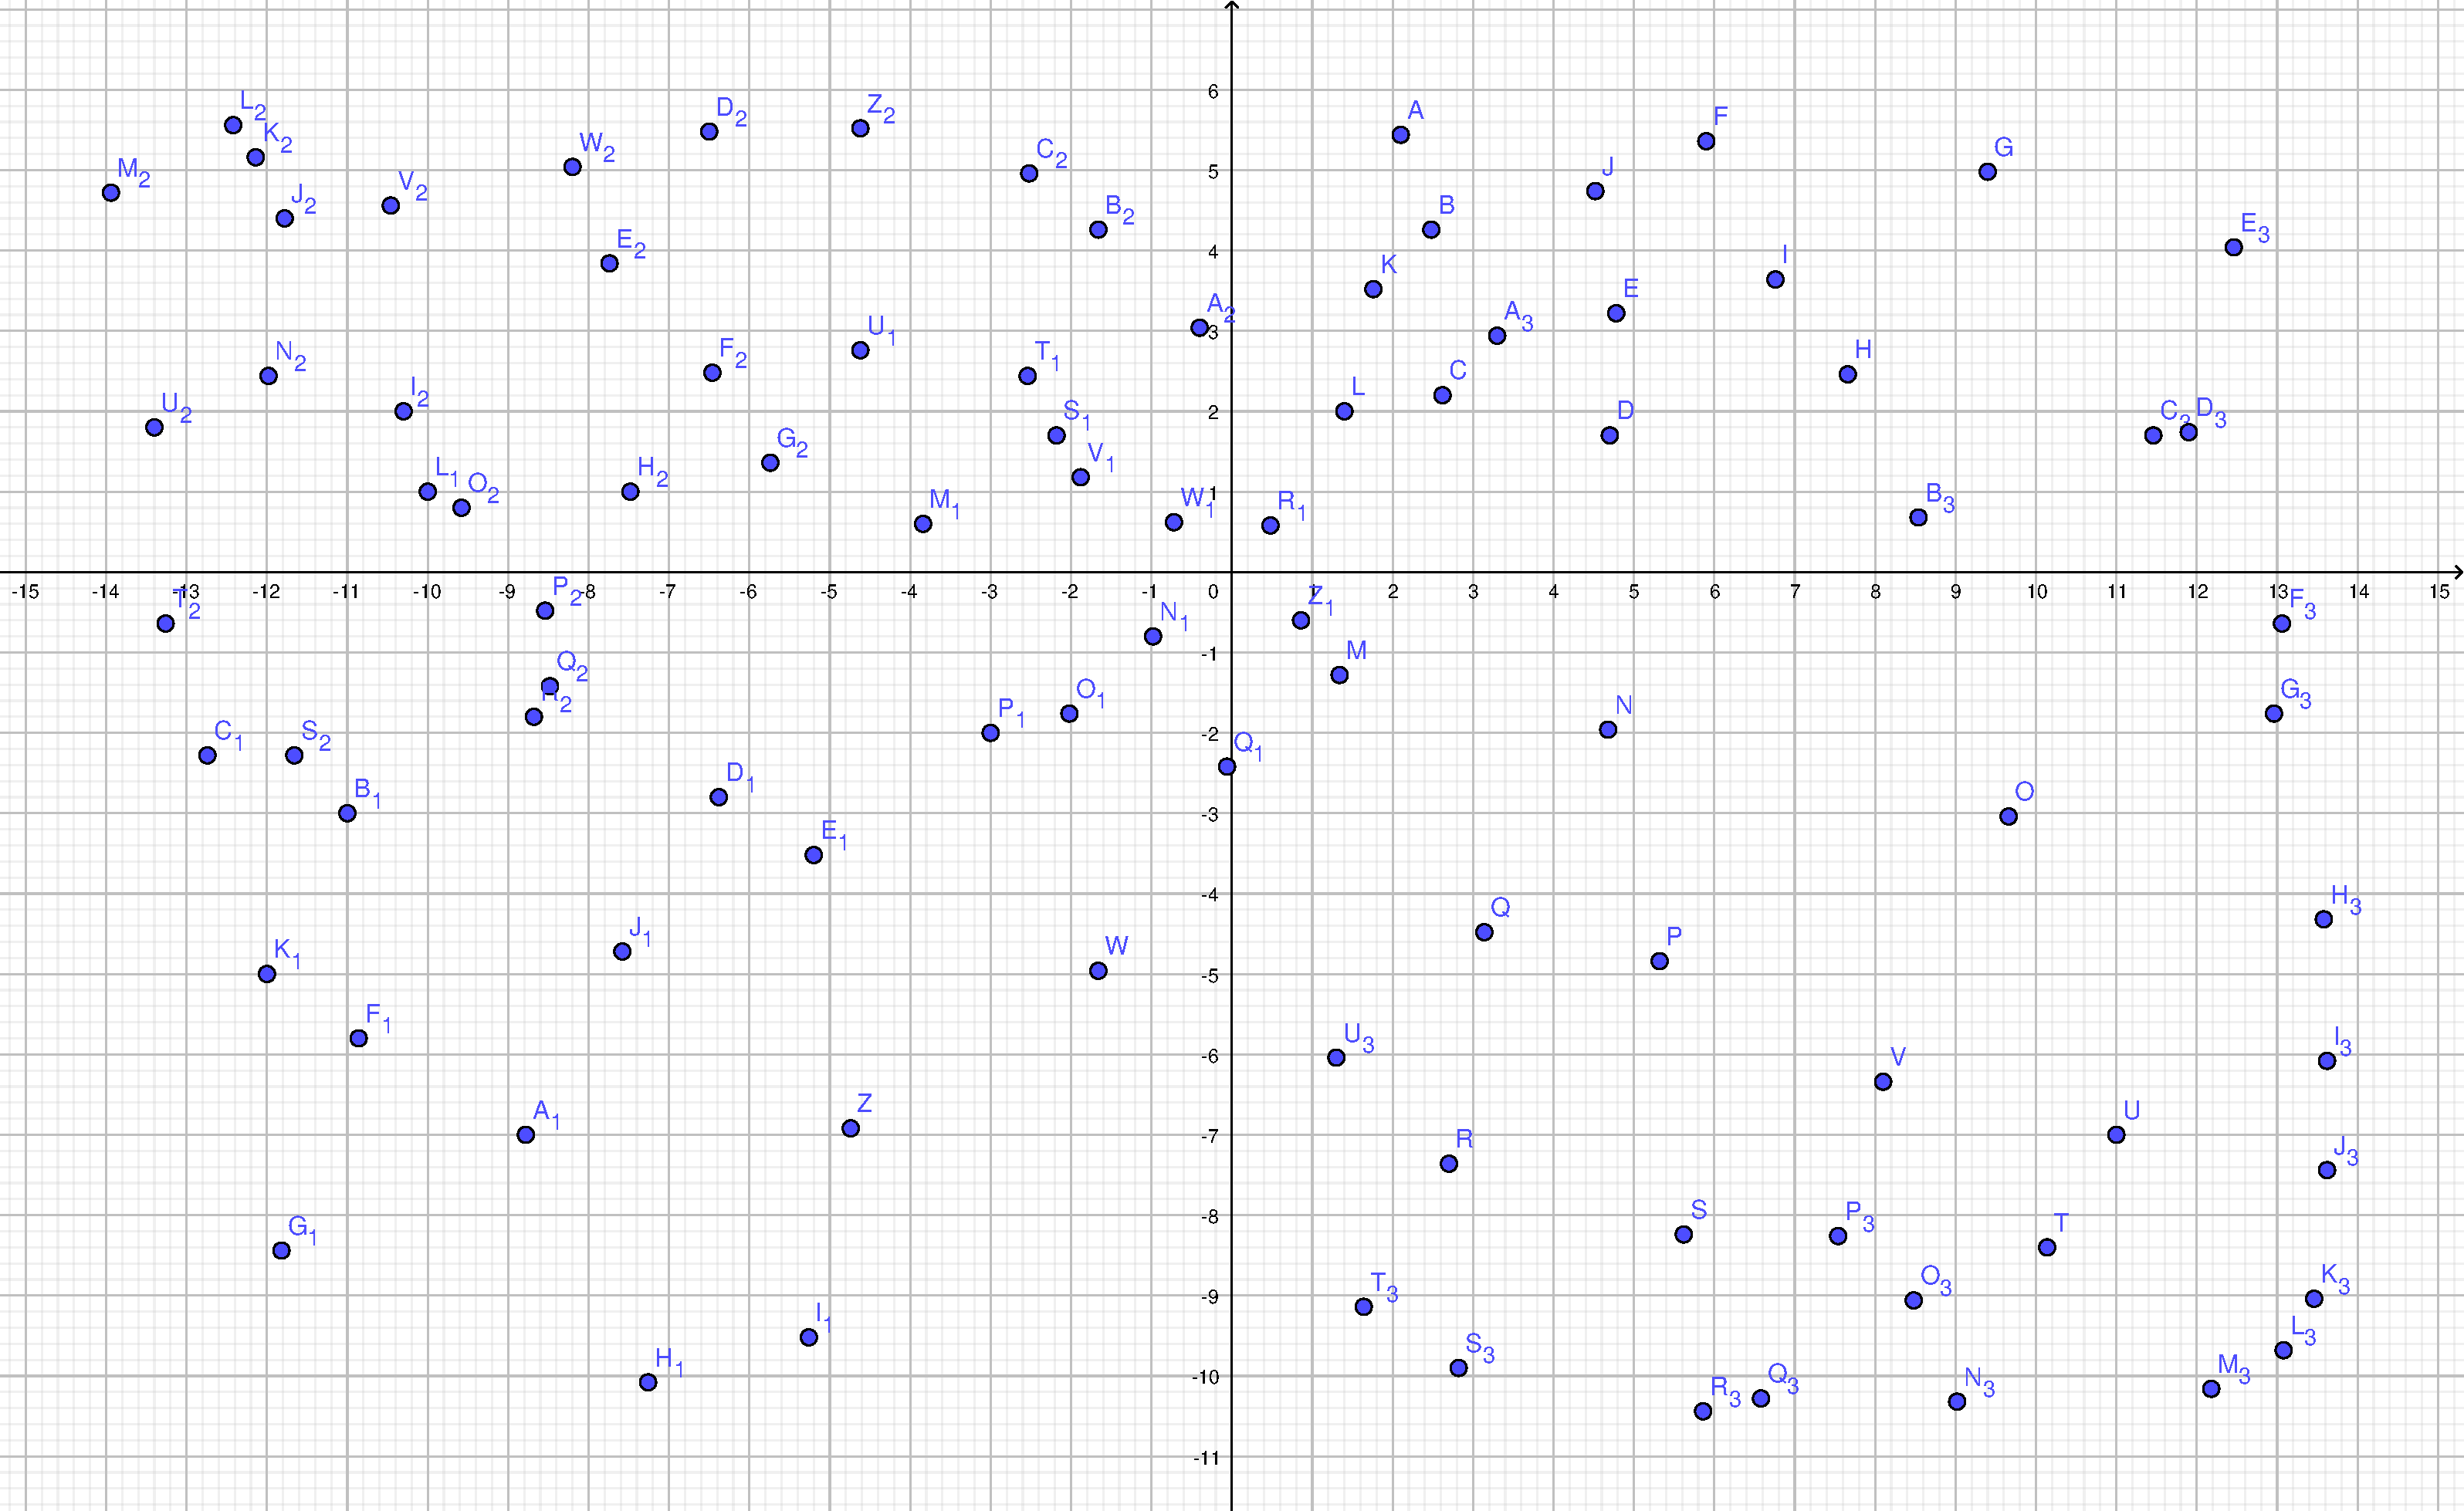
\includegraphics[width=\textwidth]{Gen-i-vyborka.pdf}
\caption{Генеральная совокупность}\label{fig:Gen-sovokup}
\end{figure}
\par
Конечно~же лучшим способом исследования генеральной совокупности является изучение всех входящих в~неё~объектов. Иногда это~не~представляет никакой сложности. Генеральная совокупность <<международные аэропорты, расположенные на~территории СПБГА>> состоит из~единственного объекта. Однако чаще всего, генеральная совокупность, во-первых достаточно велика, во-вторых, сведения о~существенной, а~чаще б\'ольшей её~части недоступны для~исследования. В~таких случаях целесообразным и~единственным способом получения знаний о~её~свойствах является формирование выборки из~данной совокупности и~её~дальнейшее изучение. Важным условием применимости выводов, полученных на~основе анализа выборки, ко~всей генеральной совокупности является её~репрезентативность, т.~е.~свойство отражать закономерности, присущие всему множеству.

\subsection{Формирование репрезентативной выборки}

Предположим, что~на~рисунке~\ref{fig:Gen-sovokup} изображена генеральная совокупность объектов, относящихся к~какому-либо сегменту рынка, всего 72~объекта. При~этом по~оси x отложена площадь объектов, по~оси y "--- их~стоимость. Простым и~корректным способом формирования выборки является т.\,н.~\emph{простая случайная выборка (\foreignlanguage{english}{simple random sample})}. При~обеспечении достаточной меры случайности отбора наблюдений и~значительного числа, выборка будет схожа с~генеральной совокупностью. На~рисунке~\ref{fig:simple-random-sample} показан пример такой случайной выборки. На~первый взгляд выборка выглядит достаточно репрезентативной. Подвидом данного метода формирования выборки является \emph{механическая выборка}. Её~отличие заключается в~том, что~первый элемент отбирается случайным образом, а~все~последующие "--- на~основе какого-либо правила. Например, случайным образом из~списка предложений выбирается одно из~них, после чего~выбираются два~наблюдения, имеющие порядковые номера, отличающиеся по~модулю от~номера первого наблюдения на~какое-либо число, после чего цикл продолжается до~получения нужного количества наблюдений. Другим вариантом является формирование \emph{стратифицированной выборки (\foreignlanguage{english}{stratified sample})}. Предположим, мы~хотим взять по~4~объекта из~каждого сектора, ограниченного осями. Если ввести предположение о~том, что~оси характеризуют среднее значение показателя, это~будет означать, что~мы хотим взять четыре~объекта, имеющих площадь и~стоимость выше средних, четыре "--- цену выше и~площадь ниже средней и~т.~д. Пример такой выборки показан на~рисунке~\ref{fig:stratified-sample}. Как~видно, данная выборка также выглядит репрезентативной. Следующим вариантом является формирование \emph{групповой выборки (\foreignlanguage{english}{cluster sample})}. В~этом случае на~первом этапе осуществляется предобработка данных, в~ходе которой формируются группы~(кластеры), включающие в~себя наиболее близкие по~тем~или~иным признакам объекты. Далее из~каждой группы отбирается определённое число наблюдений, например два. Пример групповой выборки изображён на~рисунке \ref{fig:cluster-sample}.
\par
На~первый взгляд может показаться, что~стратифицированная и~групповая выборка представляют собой один и~тот~же тип выборки. Однако, это~не~так. В~общем, можно сказать, что~примером стратифицированной выборки является отбор по~критериям цены и~площади, как~было описано выше. Примером групповой выборки является отбор наблюдений по-критерию расположения объектов в~различных районах. В~таблице \ref{tab:strat-clust-sample-diff} приведены сводные данные о~различиях между этими двумя способами формирования выборки.

\begin{table}[ht]
	\caption{Различия между групповой и~стратифицированной выборками~\cite{Studfile:strat-clust-sample-diff}}  \label{tab:strat-clust-sample-diff}
	\centering% центрируем таблицу
	\begin{tabularx}{\textwidth}{X|XX} 
		\hline
		\multicolumn{1}{c|}{} & \multicolumn{1}{c}{Групповая выборка} & \multicolumn{1}{c}{Стратифицированная выборка}  \\ 
		\hline\hline
		Охват
		& Выборка формируется только из~некоторых групп~(кластеров)
		& Выборка формируется из~всего множества 
		\\ \hline
		Требования к~однородности и~различиям
		& В~пределах группы~(кластера) элементы должны отличаться (быть разнородными), при~этом существует требование к~однородности или~схожести между различными кластерами  
		& В~пределах страты элементы должны быть однородными, тогда~как между стратами должны быть различия
		\\ \hline
		Схема выборки
		& Нужна только для~групп~(кластеров), попавших в~выборку   
		& Формируется полностью для~всех стратифицированных подмножеств
		\\ \hline
		Назначение
		& Повышает эффективность выборки, уменьшая стоимость исследования  
		& Повышает точность     
		\\ \hline
	\end{tabularx}
\end{table}
Все~рассмотренные выше способы формирования выборки относятся к~вероятностным. Существуют также детерминированные способы, с~которыми можно ознакомиться например в~\cite{FDF:types-of-sampling}.

\begin{figure}[ht]
	\centering % Центрируем картинку
	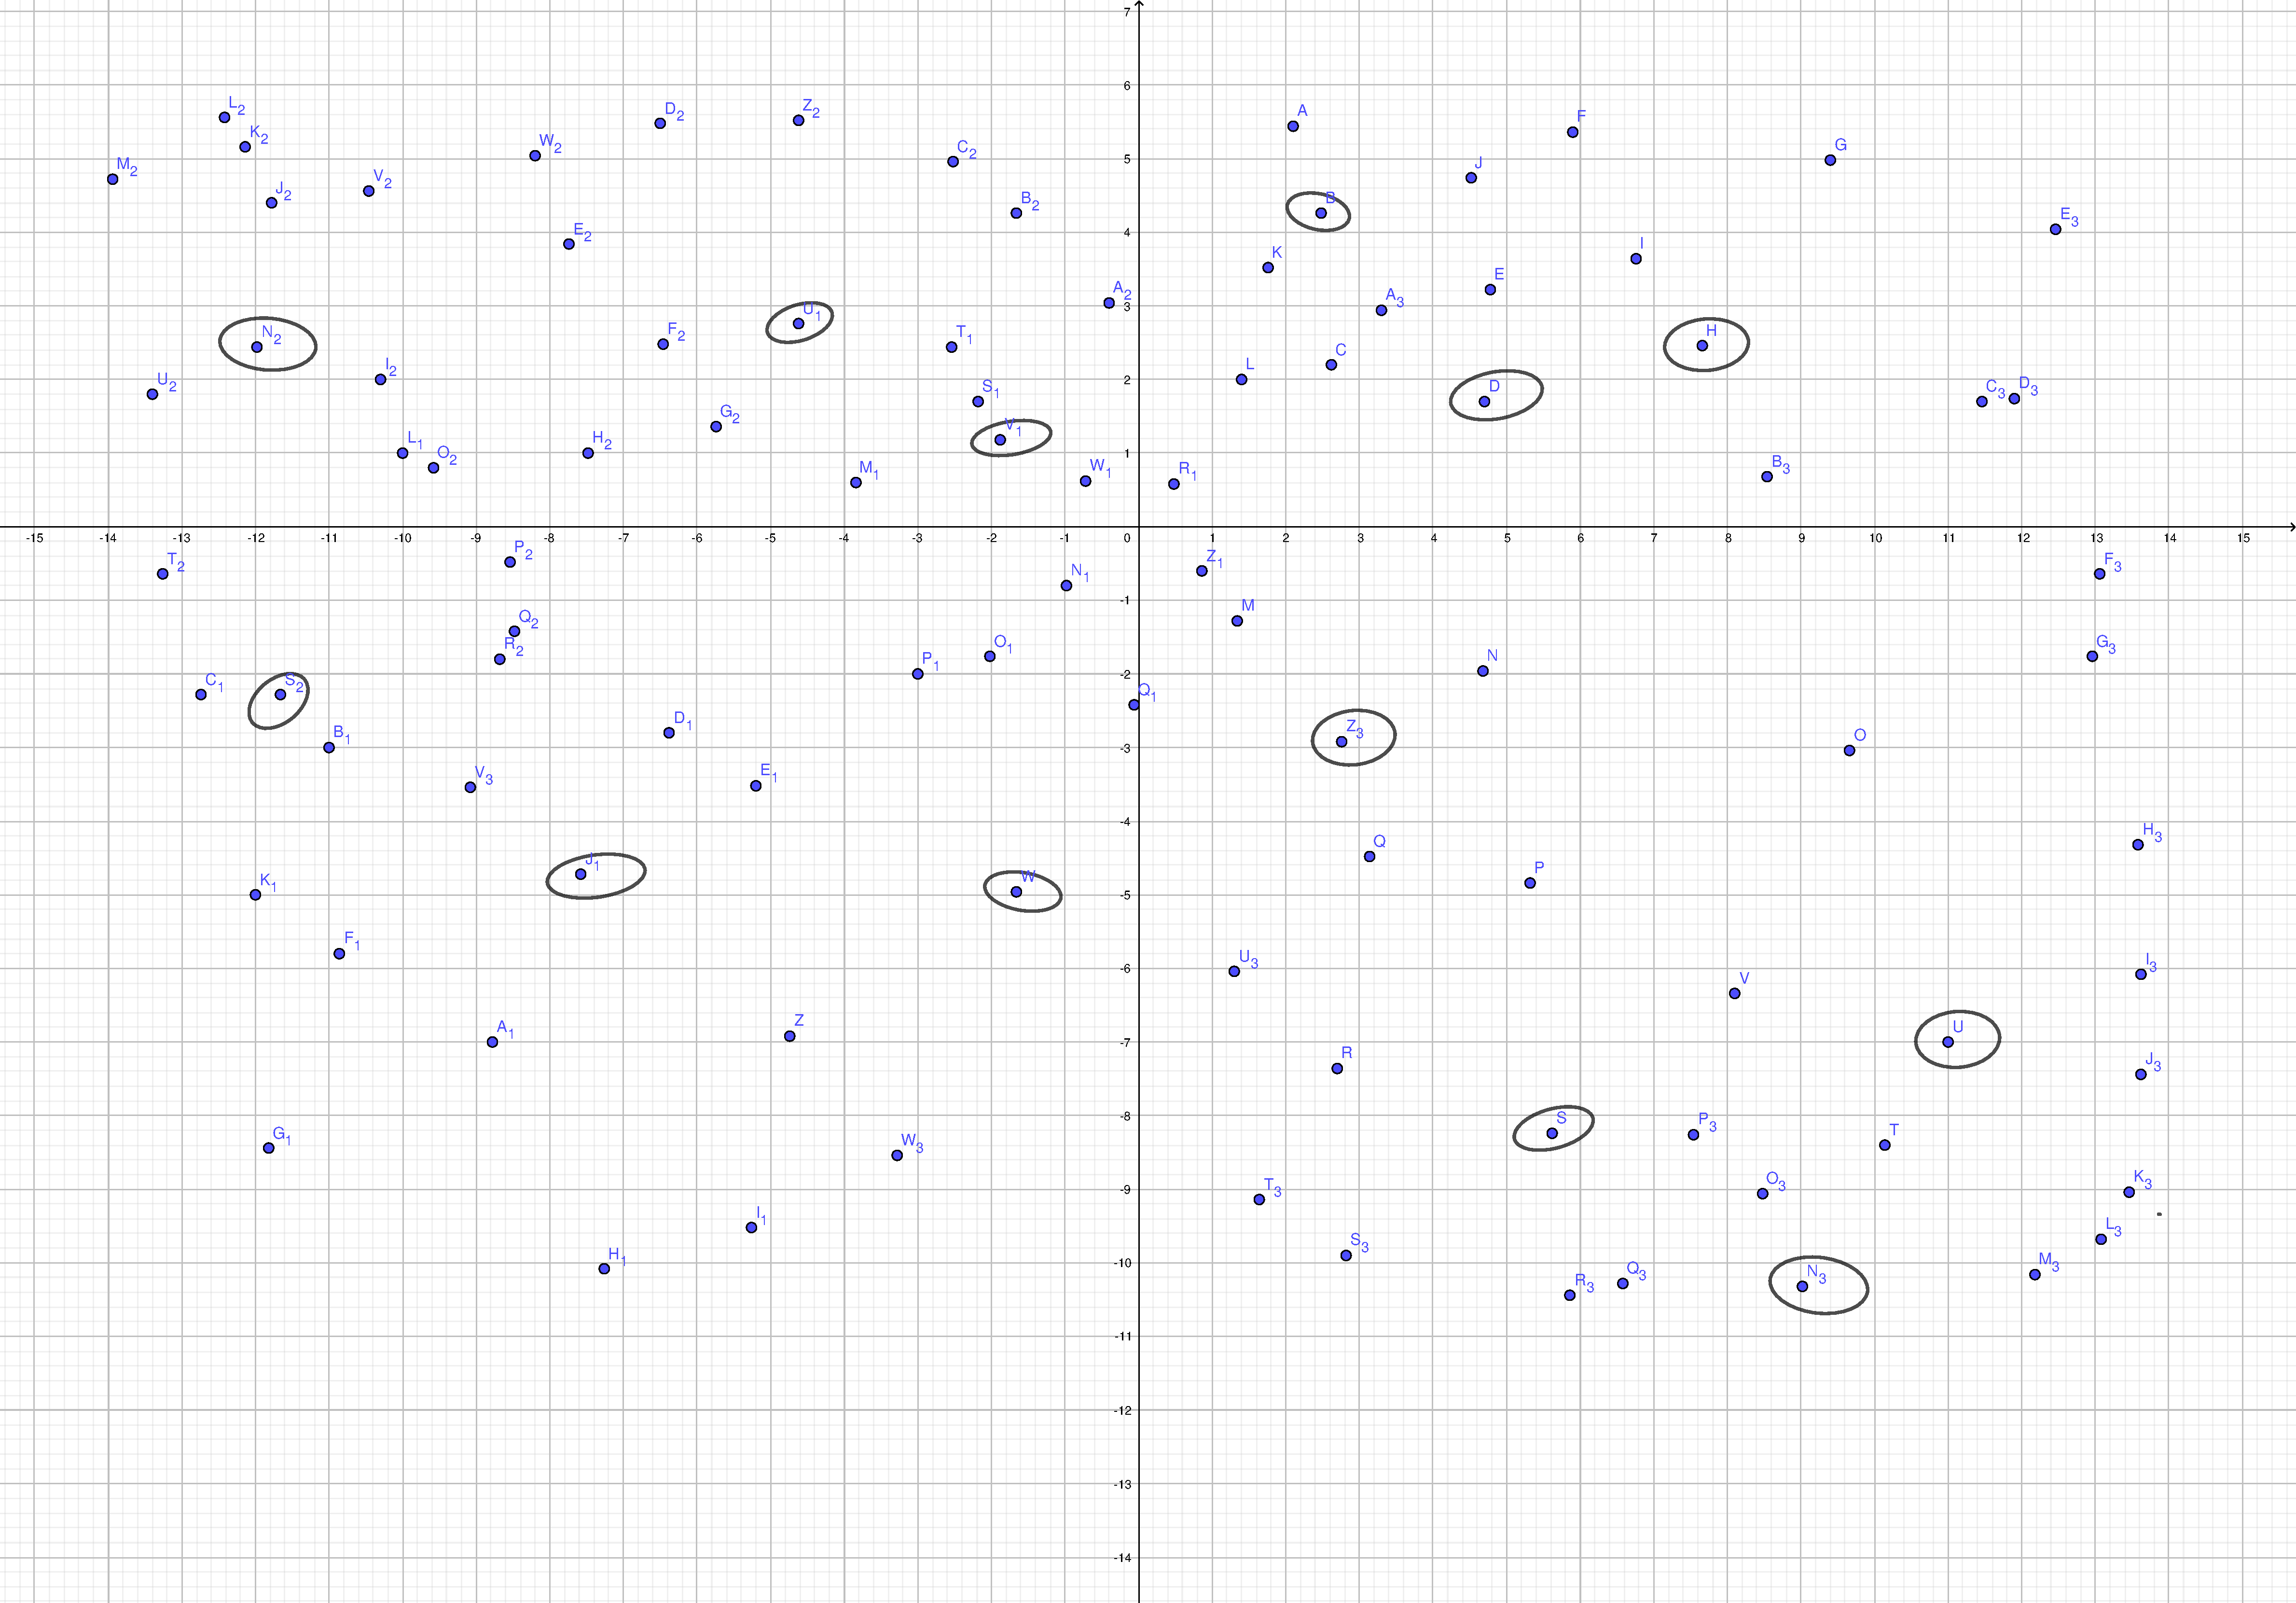
\includegraphics[width=\textwidth]{simple-random-sample.pdf}
	\caption{Простая случайная выборка}\label{fig:simple-random-sample}
\end{figure}

\begin{figure}[ht]
	\centering % Центрируем картинку
	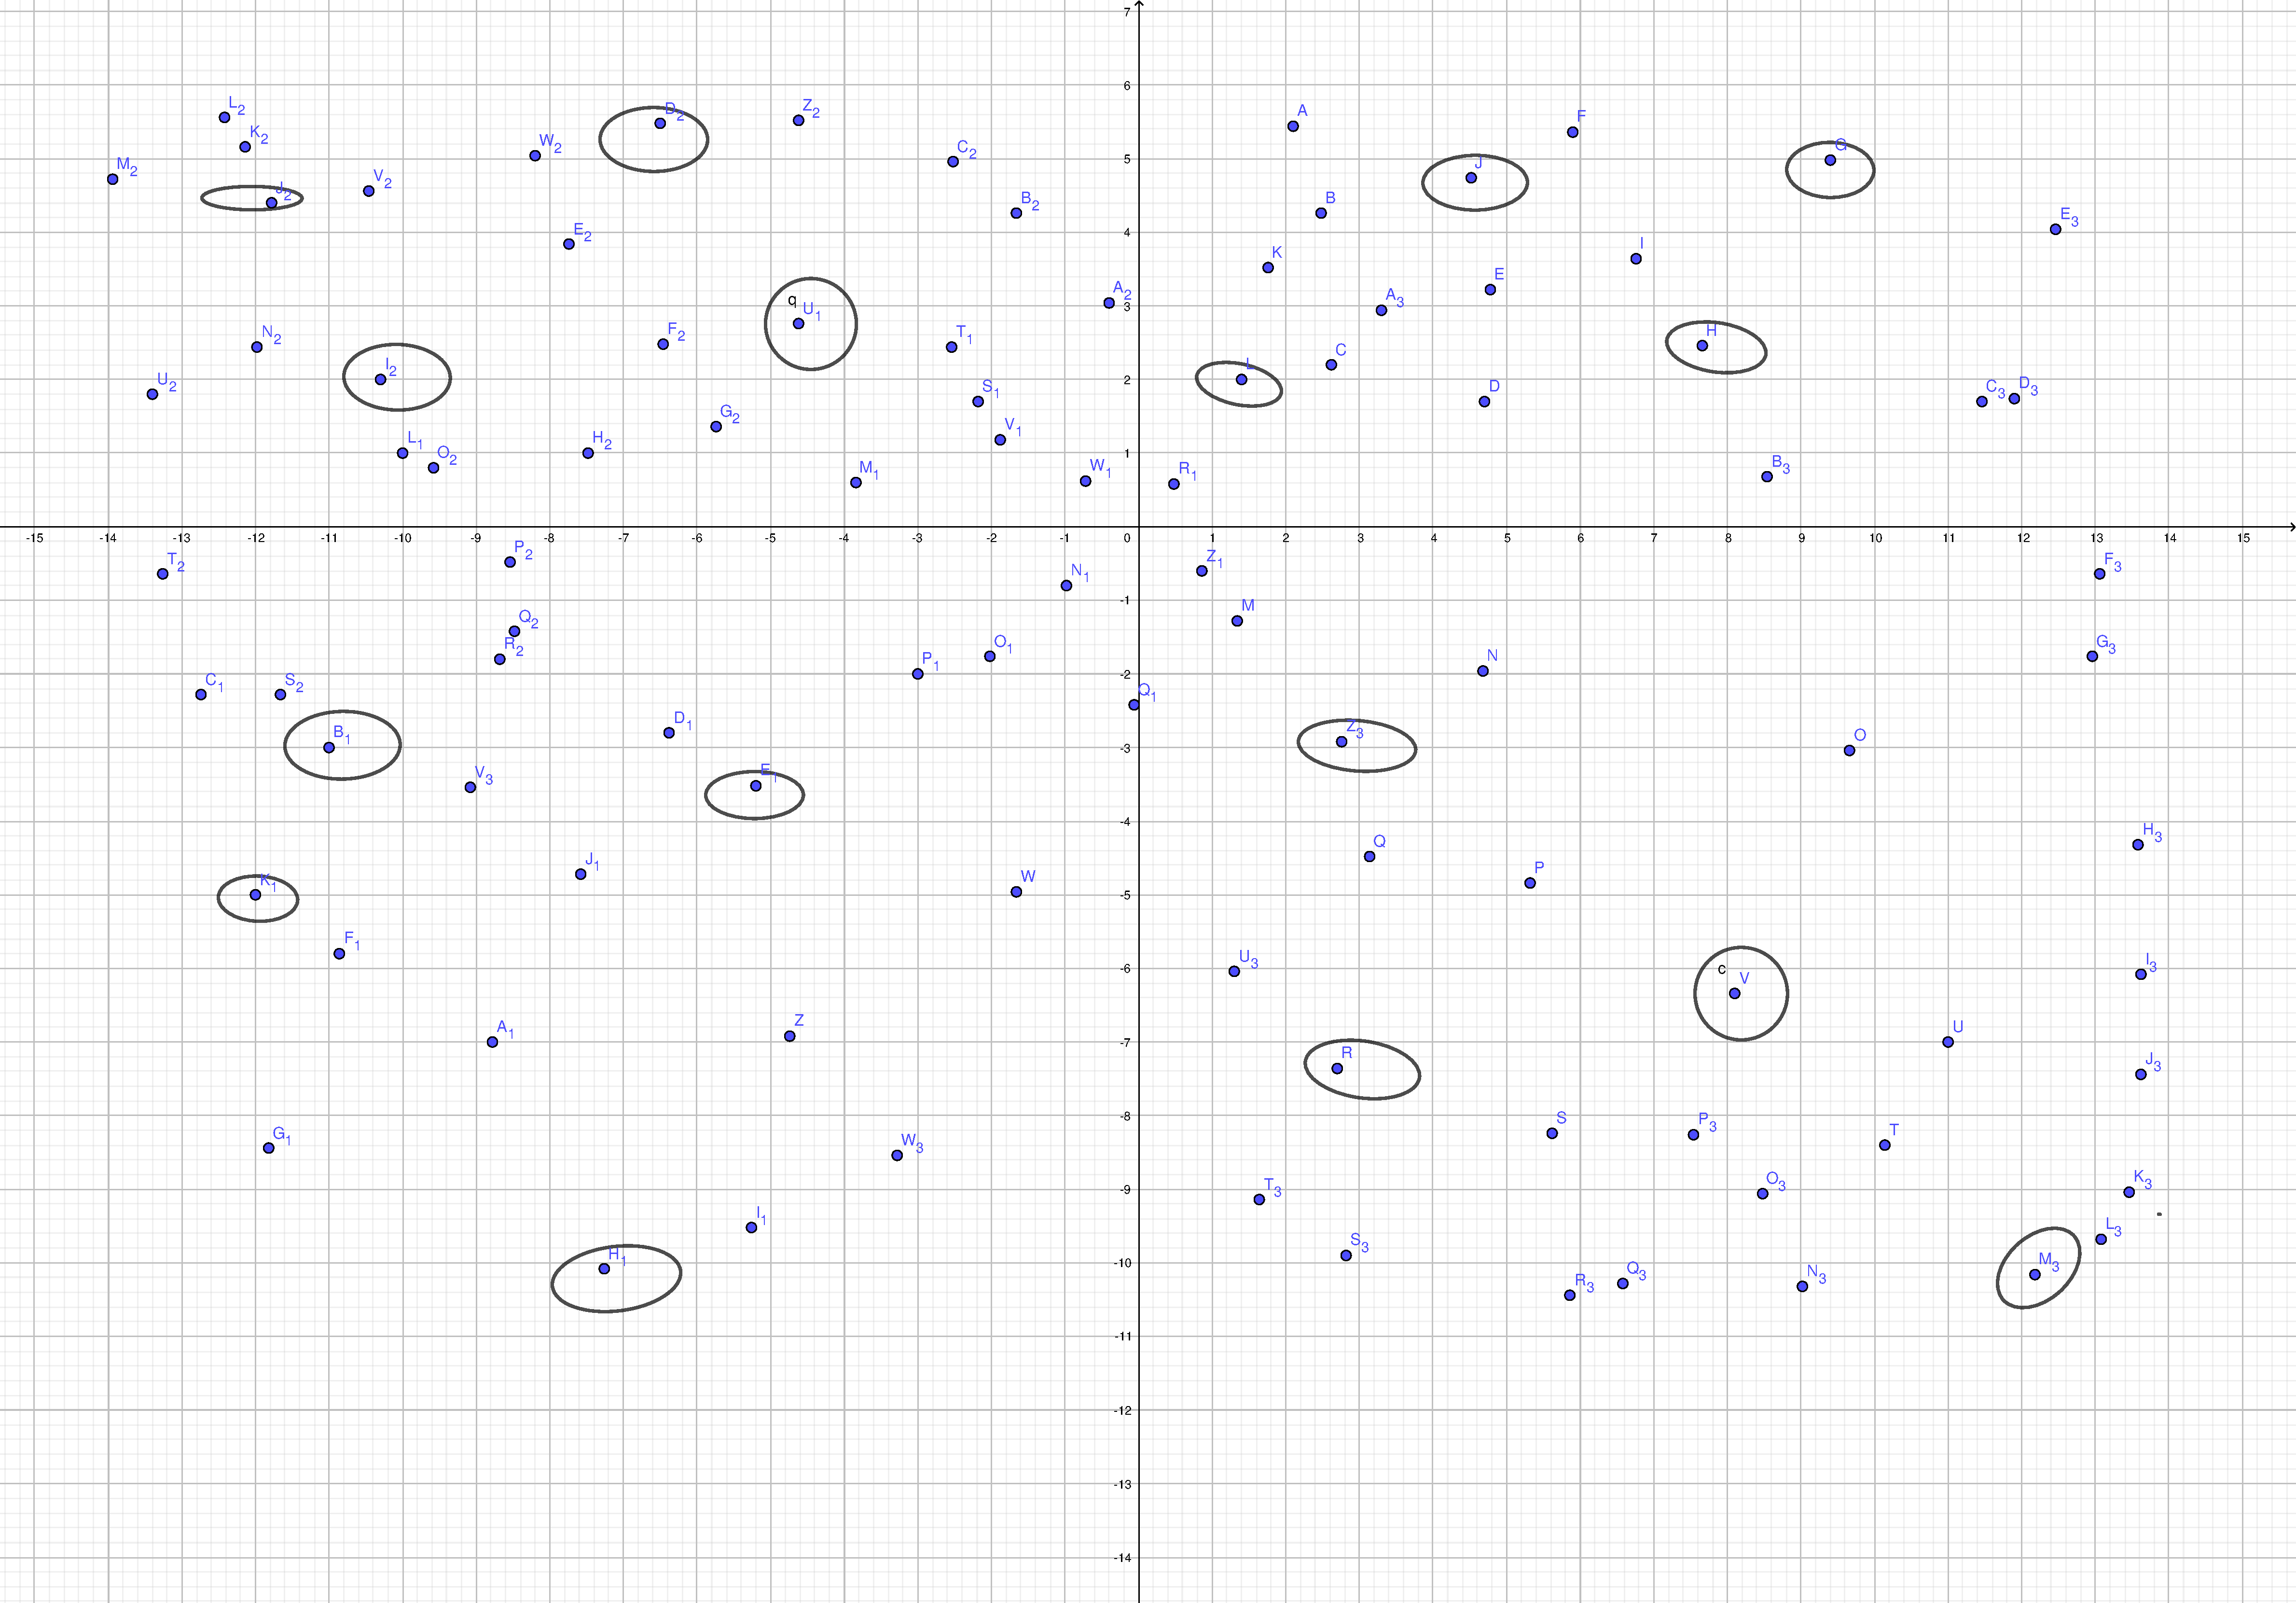
\includegraphics[width=\textwidth]{stratified-sample.pdf}
	\caption{Стратифицированная выборка}\label{fig:stratified-sample}
\end{figure}

\begin{figure}[ht]
	\centering % Центрируем картинку
	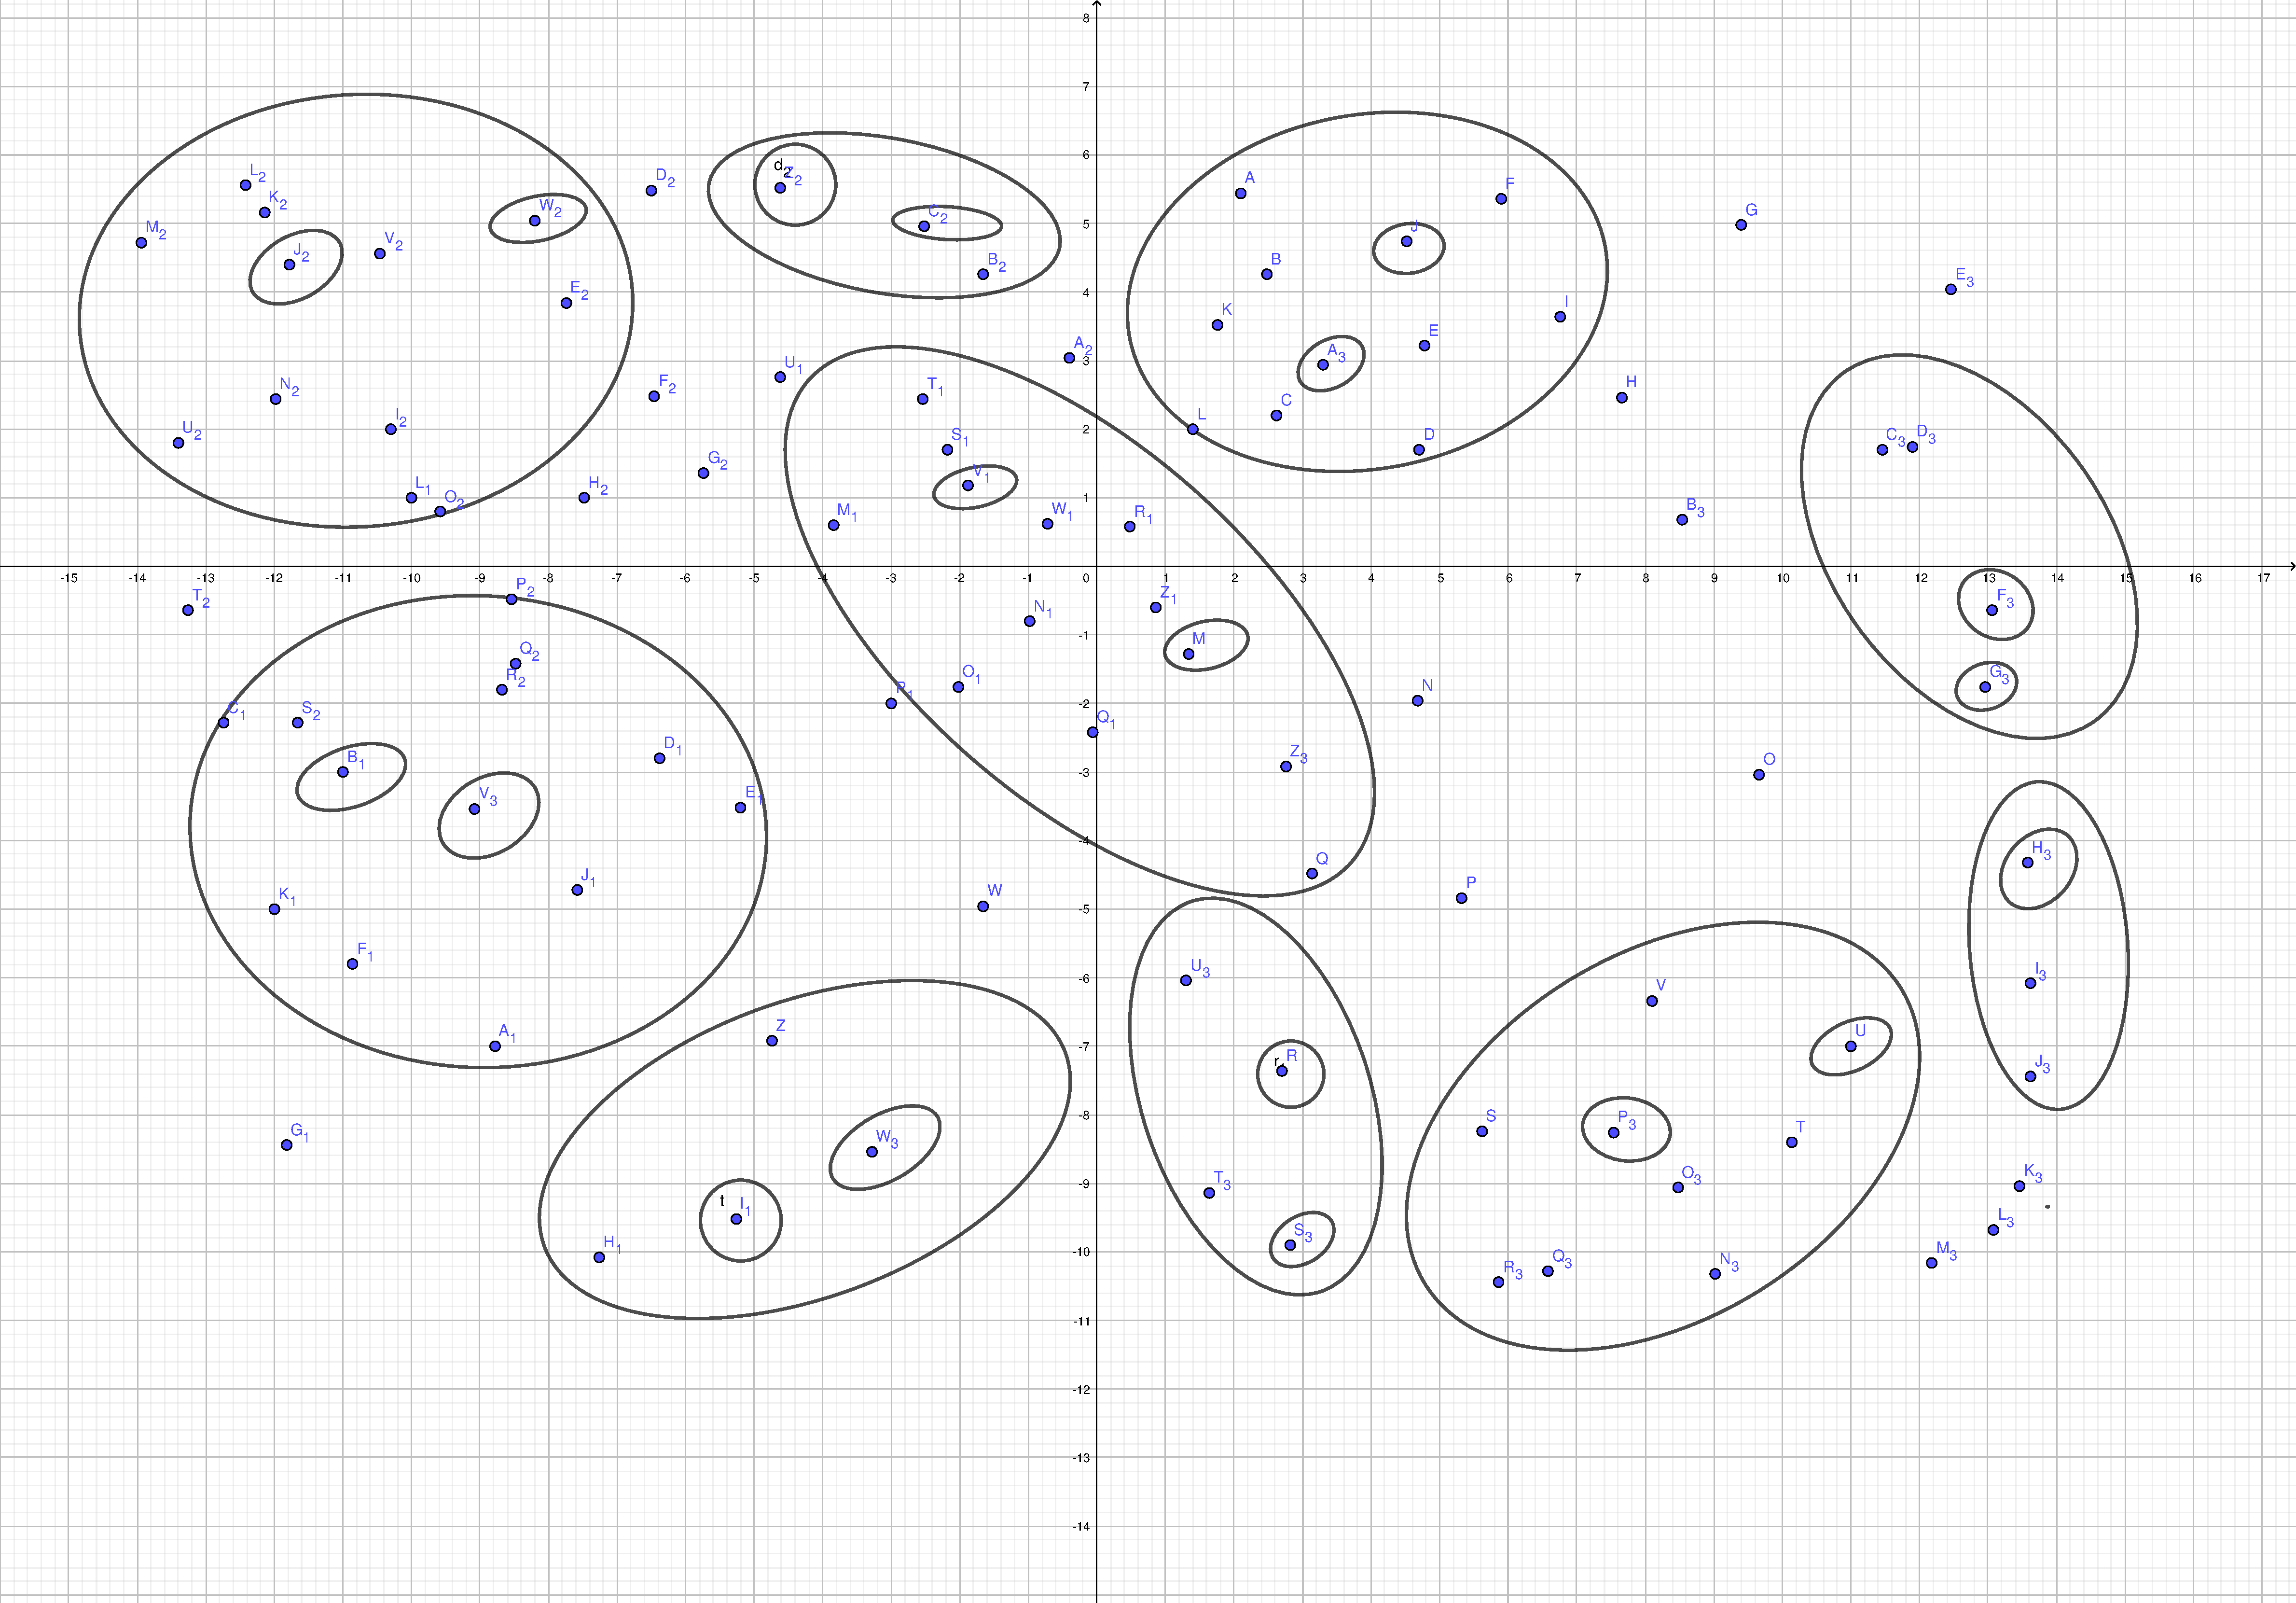
\includegraphics[width=\textwidth]{cluster-sample.pdf}
	\caption{Групповая выборка}\label{fig:cluster-sample}
\end{figure}


\section{Измерения}
Для~осуществления статистического анализа рынка необходимо преобразовать массив входящей информации в~данные. На~практике это~означает необходимость присвоения значений ключевым объектам, понятиям и~характеристикам. При~этом такое присвоение не~может носить случайный либо субъективный характер. Необходима система.
\par
Чаще всего оценщики работают с~числовыми данными, однако это~не~единственный тип данных, подлежащих анализу. Например разделения объектов, пригодных и~предназначенных для~постоянного проживания в~них людей и~домашних животных, на~квартиры и~апартаменты само по~себе не~несёт никакой числовой информации.
\par
\begin{description}
\item[Измерение] "--- это~процесс систематического присвоения количественных значений характеристикам объектов и~их~свойствам для~облегчения использования математического аппарата при~изучении и~описании объектов и~их~взаимосвязей~\cite{Statistika-dlya-vsex}.
\end{description}
Некоторые типы измерений носят вполне определённый характер: площадь земельного участка в~квадратных метрах, возраст здания в~годах, цена предложения в~рублях, пробег автомобиля в~километрах. Работа с~такими данными очень удобна: они~однозначны, могут переводиться из~одних единиц в~другую, возможно установление связи между различными переменными такого типа, например простое деление стоимости на~площадь даёт показатель стоимости за~единицу площади. Однако не~все данные изначально имеют количественную оценку. О~типах данных мы~и~поговорим далее.
\subsection{Типы данных}
Существует несколько типов данных. В~первую очередь следует сказать о~том, что~данные бывают \textbf{количественными}, \textbf{порядковыми} и~\textbf{номинативными}. Третий тип данных также называют номинальными, однако последний термин в~практике оценки прочно закрепился за~вариантом денежного потока, вследствие этого во~избежание двусмысленности оценщикам лучше придерживаться первого варианта обозначения этого типа данных.
\subsubsection{Номинативные данные}
\textbf{Номинативные данные} представляют собой метку, имя и~т.\,п.~качественные характеристики, не~имеющие смысла в~виде числа. К~таким данным относятся, например адрес объекта недвижимости (как~целиком, так~и, например в~виде метки, обозначающей муниципальное образование), его~тип, наименование завода-изготовителя промышленной установки, применяемая хозяйственным обществом система налогообложения. Мы~можем закодировать такие данные в~виде чисел, например присвоив значение <<0>> квартирам, и~<<1>> апартаментам, либо <<0>> "--- предприятиям, применяющим ОСНО, <<1>> "--- УСН <<доходы>>, <<2>> "--- УСН <<доходы, уменьшенные на~величину расходов>> и~т.\,д., однако такое присвоение является не~более чем~способом кодирования данных без~какого-либо количественного смысла. Кроме того можно переставить значения кодов и~начать присваивать <<0>> апартаментам, а~<<1>> квартирам без~потери либо искажения смысла кодирования. В~случае сомнения насчёт того, являются~ли те~или~иные данные номинативными, исследователю необходимо задать себе вопрос <<отражают~ли числа некоторое свойство так, что~более высокое значение означает наличие большего количества этого свойства?>>. В~случае отрицательного ответа можно с~уверенностью говорить о~том, что~имеют место номинативные данные. Следующим критерием отнесения данных к~номинативному типу является полная бессмысленность осуществление каких-либо арифметических действий c~числовыми метками. Несложно догадаться, что~сложение и~вычитание, не~говоря уже~об~умножении или~делении, например значений кодов ОКТМО являются по~меньшей мере бессмысленными.  Другое название данного типа "--- \textbf{категориальные данные}, что~говорит о~том, что~наличие того или~иного значения отражает принадлежность к~определённой категории, а~не~количественное измерение какого-либо свойства. Вопреки некоторым представления, такие данные вполне поддаются анализу методами частотной статистики. Особым случаем является ситуация, когда возможны лишь два значения. Такие данные называются \textbf{бинарными}. Данный случай настолько распространён и~важен, что~для~таких данных существуют особые методы анализа, например \emph{логистическая регрессия}, а~также \emph{отношение шансов} и~\emph{отношение рисков}.
\subsubsection{Порядковые данные}
\textbf{Ранговые~(порядковые) данные} "--- представляют собой данные, значения которых можно расположить в~каком-либо осмысленном порядке, таким образом что~б\'ольшие значения соответствуют большему проявлению какого-либо признака относительно меньших. Примером таких данных можно считать звёздность гостиницы. Большее число звёзд означает более высокий класс качества обслуживания гостей и~является косвенным признаком большей типичной стоимости номеров или~единицы площади самой гостиницы. При~этом категории гостиниц можно расположить в~логичной последовательности. Также оценщики часто используют порядковую шкалу для~кодирования качества и~состояние отделки объектов недвижимости.При~этом не~существует какой-либо измерительной шкалы, позволяющей определить расстояние между рангами либо ответить на~вопрос, <<является~ли оно~одинаковым между всеми соседними рангами или~нет?>>. Сами числа в~порядковых данных в~отличие от~номинативных имеют определённый смысл, существуют методы извлечения полезной информации из~таких данных. При~этом, всегда следует проявлять большую осторожность при~работе с~таким типом данных. Если в~случае с~номинативными данными вряд~ли кому-то придёт в~голову вычислять среднее значение кода ОКТМО, то~нельзя исключать вариант того, что~кто-то сочтёт возможным посчитать среднее значение для~порядковых данных, чего делать ни~в~коем случае нельзя. Вычисление среднего предполагает операцию деления, применимую только к~одному типу данных "--- \hyperref[Interval-data]{данным, характеризующим отношения}, о~которых будет сказано далее в~\ref{Interval-data}. При~этом вычисление медианы для~порядковых данных является допустимым.
\subsubsection{Количественные данные}
Количественные данные в~отличие от~номинативных либо порядковых могут быть получены непосредственно в~результате измерения. 
\paragraph{Интервальные данные и~данные, характеризующие отношения}\label{Interval-data}
\par
\textbf{Интервальные данные} характеризуются осмысленным порядком и~равными интервалами между измерениями, отражающими равновеликие изменения количества любой измеренной величины. Примером таких данных является температура, измеренная по~шкале Цельсия. Различие температуры между 20~и~40\,$\textcelsius$ такое~же, какое оно~между 40~и~60\,$\textcelsius$. Операции сложения и~вычитания являются осмысленными для~этого типа данных, поскольку разница на~единицу характеризует одинаковое изменение признака на~всём протяжении шкалы. Однако, поскольку у~шкалы Цельсия (равно как~и~у~шкалы Фаренгейта) нет~естественного нуля. Значение температуры 0\,$\textcelsius$ не~означает полное отсутствие тепловой энергии, а~является лишь удобной с~точки зрения повседневной деятельности точкой отсчёта. В~связи с~этим некорректно говорить о~том, что~40\,$\textcelsius$ означает состояние <<в~два раза теплее>> относительно 20\,$\textcelsius$. Оценщики редко могут встретиться с~таким типом данных. Единственным примером можно считать данные, описывающие параметры оборудования или~материала с~точки зрения их~жаропрочности. Для~полноценного оперирования такими значениями целесообразно перевести показатели в~градусы по~шкале Кельвина, поскольку данная шкала оперирует данными, характеризующими отношения, о~которых пойдёт речь ниже.
\par
\textbf{Данные, характеризующие отношения} обладают всеми полезными свойствами интервальных данных (осмысленный порядок, равные интервалы), но~имеют при~этом естественным ноль. Площадь, масса, хронологический возраст и~наконец сама стоимость "--- это~данные характеризующие отношения. Любые арифметические действия с~такими данными являются осмысленными.
\par
С~учётом относительной редкости интервальных данных в~данной работе в~дальнейшем всегда будут подразумеваться данные, характеризующие отношения, если прямо не~указано обратное.
\paragraph{Дискретные и~непрерывные данные}\label{Discret-data}
\par
\textbf{Дискретные данные} могут принимать только определённые значения, при~этом между этими значениями существуют чёткие границы и~равные интервалы. Количество комнат и~санузлов в~квартире, этажей в~торговом центре, входов в~помещение, число двигателей летательного аппарата или~лотков подачи сырья в~установку "--- всё~это дискретные данные.
\par
\textbf{Непрерывные данные} могут принимать любые значения в~принципе либо внутри~определённого диапазона. Расстояние, мощность, выручка "--- непрерывные данные. В~строгом общенаучном смысле можно сказать, что~почти любые непрерывные данные на~самом деле дискретные. Действительно, выручка может быть измерена с~точностью не~выше чем~до~копеек, расстояние не~более чем~с~точностью до~$\approx3\times10^{-15}$~м. То~есть в~любом случае можно говорить о~существовании некоего <<кванта>>, дробление ниже которого является невозможным. Однако на~практике чаще всего можно и~нужно пренебречь такой строгостью и~говорить о~непрерывности данных. При~этом возникает логичный вопрос, каким образом разграничить дискретные и~непрерывные данные, если между неми нет~однозначной разницы, и~в~определённом смысле практически любые данные дискретны по~своей физической природе. Не~сущесвтует однозначного и~единственно верного способа провести разграничение. Следует придерживаться стандартов анализа конкретных величин. Существует рекомендация, согласно которой данные можно считать непрерывными, если для~них~возможными являются 16~и~более значений~\cite{Statistika-dlya-vsex}. 
\subsubsection{Основные выводы}
Оценщикам не~следует забывать о~различиях между типами данных и~применять к~ним только те~арифметические действия и~методы анализа, которые являются допустимыми. Следует отметить, что~полный набор методов частотной статистики применим только в~случае непрерывных данных. В~остальных случаях следует проявлять осторожность и~использовать специальные методы, предназначенные для~других типов данных. В~отдельных случаях, проявляя осторожность, понимая смысл выполняемых операций и~осознавая ответственность за~результат, допустимо отступление от~стандартных правил. Например, можно рассчитать среднюю этажность домов в~населённом пунктке, несмотря на~то, что~число этажей не~является непрерывными данными. Распространённым примером некорректного применения статистических методов является ситуация, когда оценщики кодируют состояние объекта по~шкале, например от~1~до~5, а~затем применяют такую переменную в~качестве предиктора в~регрессионной модели, используя её~значения как~числа. Компьютер само собой не~знает о~том, что~на~самом деле ему~в~обработку была передана не~количественная, а~порядковая переменная и~начинает честно считать среднее значение, сравнивать с~ним значения каждого наблюдения и~т.~д. В~итоге, такая модель, хотя и~выглядит наукообразно, на~самом деле несёт в~себе искажение информации и~вряд~ли может использоваться в~серьёзном анализе. В~целом, данная проблема не~является специфичной для~оценки. Известная всем со~школы система расчёта среднего балла также является  антинаучной, равно как~и~система потолка оценок, при~которой талантливые ученики не~могут получить балл выше <<5>>, даже если их~уровень намного превышает тот, который по~умолчанию соответствует высшей оценке. К~сожалению, в~мире по-прежнему много пережитков мрачного прошлого, а~Знание не~всегда побеждает архаику тёмных времён. На~данном этапе развития оценочной деятельности особенно важно придерживаться научных принципов, не~использовать сомнительные приёмы, лишь на~первый взгляд облегчающие работу. На~самом деле нет~никакой сложности в~том, чтобы корректно включить, например ранговую переменную, в~регрессионную модель. Достаточно преобразовать переменную в~фактор, после чего компьютер корректно учтёт её. Языки программирования R и~Python позволяют осуществлять подобные преобразования путём написания кода длиной в~одну четвёртую строки, см.~листинги~\ref{listing-convert-to-factor-R-1},~\ref{listing-convert-to-factor-Python-1}. Общие сведения о~допустимых и~недопустимых действиях в~отношении данных, относящихся к~одному из~рассмотренный выше типов, приведены в~таблице~\ref{tab:calculations-for-diff-data}.
\begin{table}[ht]
	\caption{Допустимые действия и~вычисляемые значения для~различных типов данных}  \label{tab:calculations-for-diff-data}
	\centering% центрируем таблицу
	\begin{tabularx}{\textwidth}{X|XXXXXX} 
		\hline
		\multicolumn{1}{c|}{} & \multicolumn{1}{c}{Частотный анализ} & \multicolumn{1}{c}{$+, - $} & \multicolumn{1}{c}{$\times, /$} & \multicolumn{1}{c}{Мода} & \multicolumn{1}{c}{Медиана} & \multicolumn{1}{c}{Среднее} \\
		\hline\hline
		Номинативные
		& да
		& нет
		& нет
		& да
		& нет
		& нет		
		\\ \hline
		Порядковые
		& да
		& вычитание
		& нет
		& да
		& да
		& нет
		\\ \hline
		Дискретные
		& да
		& да
		& нет
		& да
		& да
		& нет
		\\ \hline
		Непрерывные
		& да
		& да
		& да
		& да
		& да
		& да     
		\\ \hline
	\end{tabularx}
\end{table}

\begin{lstlisting}[float, caption = Преобразование переменной в~фактор на~языке R, firstnumber=1, language = R, label= listing-convert-to-factor-R-1]
df$col <- as.factor(df$col)
\end{lstlisting}

\begin{lstlisting}[float, caption = Преобразование переменной в~фактор на~языке Python, firstnumber=1, language = Python, label = listing-convert-to-factor-Python-1]
df[col] = df[col].astype('category')
\end{lstlisting}

\subsection{Некоторые аспекты и~проблемы измерений}
Практикам в~области анализа данных хорошо известно, что~чаще всего само моделирование связанные с~ним действия, занимают примерно 20~\% времени, тогда как~80~\% уходят на~планирование исследования, сбор и~предобработку данных. Одним из~этапов планирования является \emph{операционализация} "---  процесс определения способа описания и~измерения признаков. Операционализация необходима тогда, когда какие-либо признаки не~являются количественными либо по~иным причинам не~могут быть измерены напрямую. Определение способа кодирования, выбор числа возможных значений "--- всё~это является важной составляющей планирования сбора данных и~его реализации.
\par
Во~многих случаях необходимый признак не~может быть измерен напрямую. В~таких случаях можно использовать \emph{опосредованное измерение}, т.\,е.~заменить одном измерение другим. Например, чаще всего нет~возможности определить износ станка инструментальными методами. Вместо этого можно провести измерения его~наработки в~моточасах.

\section{Описательные статистики}
Важным этапом анализа данных рынка является их~первичная интерпретация, позволяющая сделать выводы и~разработать план исследования. Форма распределения, наличие выбросов, асимметрия, присутствие выраженных центров плотности "--- всё~это является важной информацией, позволяющей
опытному аналитику сразу~же сделать выводы, необходимые для~быстрой оценки свойств изучаемого явления либо сегмента открытого рынка.  Эволюционно мозг человека устроен таким
образом, что~от~60~до~80 процентов информации поступает в~него по~визуальному каналу и~лишь
около~10 процентов по~каналу, который можно назвать <<смысловым>>. Подробнее с~этим и~другими
выводами, описывающими основы мышления  можно ознакомиться, например в~работе бывшего руководителя Нидерладского института головного мозга Дика Свааба <<Мы "--- это~наш~мозг: от~матки до~Альцгеймера>>~\cite{Swaab:mozg}. Для~целей данной работы это~означает, что~не~следует пренебрегать визуализацией анализируемых информации. Менее наглядными, но~ещё~более важными являются составление описательных статистик и~проверка гипотезы нормальности распределения данных. Эти~три операции лежат в~основе любого первичного анализа данных открытых рынков.
\par В~данном фрагменте в~качестве примера были использованы данные из~набора \emph{<<almaty-apts-2019-1>>}~\cite{ds:almaty-apts-2019-1}, содержащего сведения о~2355 предложения в~г.~Алматы. Данный набор был любезно предоставлен казахстанской коллегой Г.~Шуленбаевой, за~что~автор выражает ей~признательность. Выбор этого набора данных обусловлен тем, что~предметом интереса настоящей работы является частотная статистика, основанная на~предпосылках о~случайности как~объективном свойстве объектов, процессов и~явлений, а~также об~отсутствии априорно известных свойств. Автор никогда не~был в~г.~Алматы и~ничего не~знает о~рынке квартир там, что~соответствует вышеуказанной предпосылке. 
\subsection{Визуализация данных}
В~данном подразделе будут рассмотрены следующие способы визуализации данных:
	\begin{itemize}
		\item гистограмма;
		\item ядерная оценка плотности;
		\item ящик с~усами~(boxplot);
		\item диаграмма рассеяния.
	\end{itemize}
\subsubsection{Построение гистограмм}
\paragraph{Основные сведения}
\par
Гистограмма "--- способ визуального отображения функции плотности вероятности вектора данных. Из~этого следует, что гистограмма является способом графического отображения распределения данных (значений случайной величины). Частотность~событий откладывается по~вертикальной оси, группы данных "--- по~горизонтальной. Полосы столбцов имеют одинаковую ширину.
\par 
Рассмотрим алгоритм её~построения. Предположим, что мы~имеем $n$ наблюдений, содержащих числовые значения $x_{1}\ldots x_{n}$. Возьмём интервал $[a, b]$, содержащий все эти числа. Разбиваем его~на~$k$ частей. Вопрос нахождения оптимального значения $k$ до~сих~пор является научной проблемой. Некоторые её~аспекты и~предлагаемые пути решения приведены в~\ref{hist-number-of-k}. Второй проблемой является проблема выбора: должны~ли эти~части содержать строго одинаковое число наблюдений. На~основании эмпирических данных и~собственного опыта автор пришёл к~выводу о~том, что~на~стадии предварительного анализа данных и~их~визуализации строгое выдерживание одинаковости количества наблюдений в~одном интервале не~носит обязательный характер, вследствие чего нет~необходимости применять процедуры, обеспечивающие выполнение такого требования. Однако по~мере возможности следует придерживаться одинаковости срединных интервалов, при~необходимости уменьшая число наблюдений в~двух крайних так, чтобы в~них оставалось не~менее 5~наблюдений~\cite{Nowiczkij:oczenka-pogresh}. Созданные части обязательно должны быть непересекающимися. Обозначим их~как~$\Delta_{1}\ldots \Delta_{k}$. Вследствие этого возникает числовая ось, имеющая границы $[a, b]$ и~состоящая из~$k$ непересекающихся частей. Затем путём простого деления
\begin{equation}\label{hist-simple}
\frac{n}{k},
\end{equation}
где $n$ "--- число наблюдений,

$k$ "--- количество частей, на которые разбиты наблюдения,
\par
определяется число наблюдений, попавших в каждую часть. Далее на~прямой $a\ldots b$ строят прямоугольники, высота $h$ которых может быть пропорциональна количеству наблюдений, попавших в~отрезок.
\begin{equation}\label{eq:hist-simple-prop}
h_{i} \propto n_{i},
\end{equation}
где $n$ "--- число наблюдений,

$i$ "--- номер части. 

Данный подход к~построению гистограммы является интуитивным, однако он~не~в~полной мере отражает вероятностную суть данного способа визуализации.

Более научный вероятностный подход гласит, что
\begin{equation}\label{eq:hist-scienced}
\frac{n_{i}}{n \times |\Delta{i}|},
\end{equation}
где~$n_{i}$ "--- число наблюдений в~i-той части,

$i$ "--- номер части,

$n$ "--- общее число наблюдений,

$\Delta_{i}$ "--- шаг разбиения.

Использование данной формулы обеспечивает выполнение условия равенства суммы площадей всех
прямоугольников единице и~является необходимым с~точки зрения обеспечения возможности сравнивать гистограммы, построенные на~выборках с~разным количеством наблюдений, тогда как~в~случае определения высоты столбцов по~формуле~\ref{eq:hist-simple-prop} она~будет зависеть от~свойств конкретного единичного набора данных.
Второй довод в~пользу использования формулы \ref{eq:hist-scienced} заключается в~следующем. В~силу равенства суммы площадей прямоугольников единице, данный способ обеспечивает отображение плотности распределения вероятности значений наблюдений.
В~таком случае можно, хоть~и~не~в~явном виде, говорить о~возможности определения вероятности того, что~измеряемые нами значения наблюдений попадут в~интервал $[a, b]$. В~этом случае получается, что~данная вероятность может быть рассчитана как~интеграл от~плотности вероятности.
\begin{equation}\label{eq:prob-integral}
P(x \in [a, b]) = \int \limits_{a}^{b} f (t)dt
\end{equation}
По~мере увеличения числа наблюдений и~в~случае правильного выбора $k$ гистограмма будет всё~меньше отличаться от~функции плотности.

Ключевым моментом при~восприятии гистограммы должно быть то, что~при~её~анализе мы смотрим на~площади. Если вычислить сумму площадей прямоугольников, расположенных на~отрезке оси абсцисс $\alpha \ldots \beta$, это~будет означать, что~мы~определили вероятность того, что значение случайной величины будет находиться в~диапазоне~$\alpha \ldots \beta$. Разумеется данное утверждение является справедливым только в~случае использование формулы~\ref{eq:hist-scienced} для~определения высоты столбцов.

При~этом следует отметить, что~использование формулы \ref{eq:hist-simple-prop} может быть оправдано в~случаях подготовки гистограмм в~презентационных и~маркетинговых целях. В~целях анализа данных осмысленным является использование исключительно формулы~\ref{eq:hist-scienced}.
\paragraph{Выбор рационального числа интервалов}\label{hist-number-of-k}
\par
Число интервалов~($k$), используемое при~вычислении оценок параметров и~построении гистограмм, колеблется в~широких пределах. Большинство рекомендуемых формул носят эмпирический характер и~часто дают завышенные значения. В~общем случае можно говорить о~том, что~количество интервалов~$k$ связано с~количеством наблюдений переменной. При~слишком малом~$k$ гистограмма будет отличаться от~действительной кривой плотности вследствие слишком крупной ступенчатости, из-за чего будет потеряна информация об~особенностях распределения. Так, если представить ситуацию, при~которой интервал группировки равен размаху, гистограмма любого распределения будет выглядеть так, как~будто имеет место равномерное распределение. В~случае с~тремя~интервалами любое колоколообразное распределение будет сведено к~треугольному. При~этом в~случае слишком большого значения $k$ гистограмма будет содержать не~только полезную информацию, но~и~значительную долю <<шума>>. Таким образом, необходимо найти баланс, который обеспечит сохранение <<сигнала>>, отсеяв при~этом <<шум>>. Таким образом, задача поиска $k$ при~построении гистограммы сводится к~\emph{задаче оптимальной фильтрации}, а~оптимальным значением $k$ является такое, при~котором максимально возможное сохранение <<сигнала>> сочетается с~максимальной возможной фильтрацией <<шума>>, иными словами, максимальное сглаживание флуктуаций должно сочетаться с~минимальным искажением кривой плотности распределения. Одним из~практических признаков приближения к~оптимальному $k$ является исчезновение <<пиков>> и~<<провалов>>, а~ближайшим к~оптимальному может считаться такое максимальное значение $k$, при~котором гистограмма ещё~сохраняет плавный характер. На~практике можно сформулировать просто правило: при~$n > 200$ каждый столбец должен содержать не~менее 10~наблюдений. При~$n \leq 200$ крайние столбцы могут содержать не~менее 5~наблюдений.  Значительное число рекомендаций по~выбору числа~$k$ из~различных источников содержится в~\cite{Nowiczkij:oczenka-pogresh}. 

В~целом можно сказать, что~существует пять групп методов определения оптимального значения $k$:
	\begin{itemize}
		\item обобщённые;
		\item основанные на~значении $n$;
		\item основанные на~критерии согласия $\chi^{2}$;
		\item основанные на~энтропийном коэффициенте;
		\item основанные на~четвёртом центральном моменте.
	\end{itemize}
\subparagraph{Обобщённые методы определения числа $k$}\label{k-hist:common-methods}
\par
В~первом приближении можно использовать рекомендацию, данную в~\cite{Shtorm:MathStat}, и~говорить о~том, что
\begin{equation}\label{n-k-Nowiczkij-1}
6 \leq k \leq 20.
\end{equation}
Также существует ещё~более обобщённая рекомендация
\begin{equation}\label{n-k-Nowiczkij-2}
k = 12 \pm 2 \ldots 3.
\end{equation}
Данные методы являются оценочными и~могут служить лишь ориентиром при~первом знакомстве с~данными.
\subparagraph{Методы определения числа $k$ на~основе $n$}\label{k-hist:n-methods}
\par
Первая формула, основанная на~числе $n$ была предложена Гербертом Стёрджессом в~1926 году в~работе~\cite{Sturgess:hist-intervals}
\begin{equation}\label{eq:hist_Sturgess-1}
k = \frac{range}{1 + \log_2 n},
\end{equation}
где \foreignlanguage{english}{range} "--- размах,

n "--- число наблюдений.

В~той~же работе были предложены формулы:
\begin{equation}\label{eq:hist_Sturgess-2}
k = 1 + \log_2 n,
\end{equation}
%
\begin{equation}\label{eq:hist_Sturgess-3}
k = 1 + 3.3\lg n,
\end{equation}
Следует отметить, что~значения, получаемые на~основе формул~\ref{eq:hist_Sturgess-2} и~\ref{eq:hist_Sturgess-3} приблизительно равны между собой
\begin{equation}\label{eq:hist_Sturgess-2+3}
1 + \log_2 n \approx 1 + 3.3\lg n.
\end{equation}
Некоторые рассуждения, касающиеся данных формул, приведены в~\cite{Wand:Data-Based-Hist}.
В~работе~\cite{Shtorm:MathStat} без~ссылки на~первоисточник предлагается формула Брукса и~Каррузера
\begin{equation}\label{eq:hist-Bruks-Karruzer}
k = 5 \lg n.
\end{equation}
В~1965 году в~книге~\cite{Ingenieur-Statistik} И.~Хайнхольд и~К.~Гаеде указывают соотношение
\begin{equation}\label{eq:hist_Heinholds-Gaede}
k = \sqrt{n}.
\end{equation}
На~рисунках \ref{fig:k-hist-n1},~\ref{fig:k-hist-n2} показан прирост $k$ при~$n < 400$ и~при~$ n < 50000$ соответственно.
\begin{figure}[ht]
	\centering % Центрируем картинку
	\includegraphics[width=\textwidth]{k-hist-1.pdf}
	\caption{Визуализация числа~k при~$n < 400$ в~случае использования методов, основанных на~значении $n$}\label{fig:k-hist-n1}
\end{figure}

\begin{figure}[ht]
	\centering % Центрируем картинку
	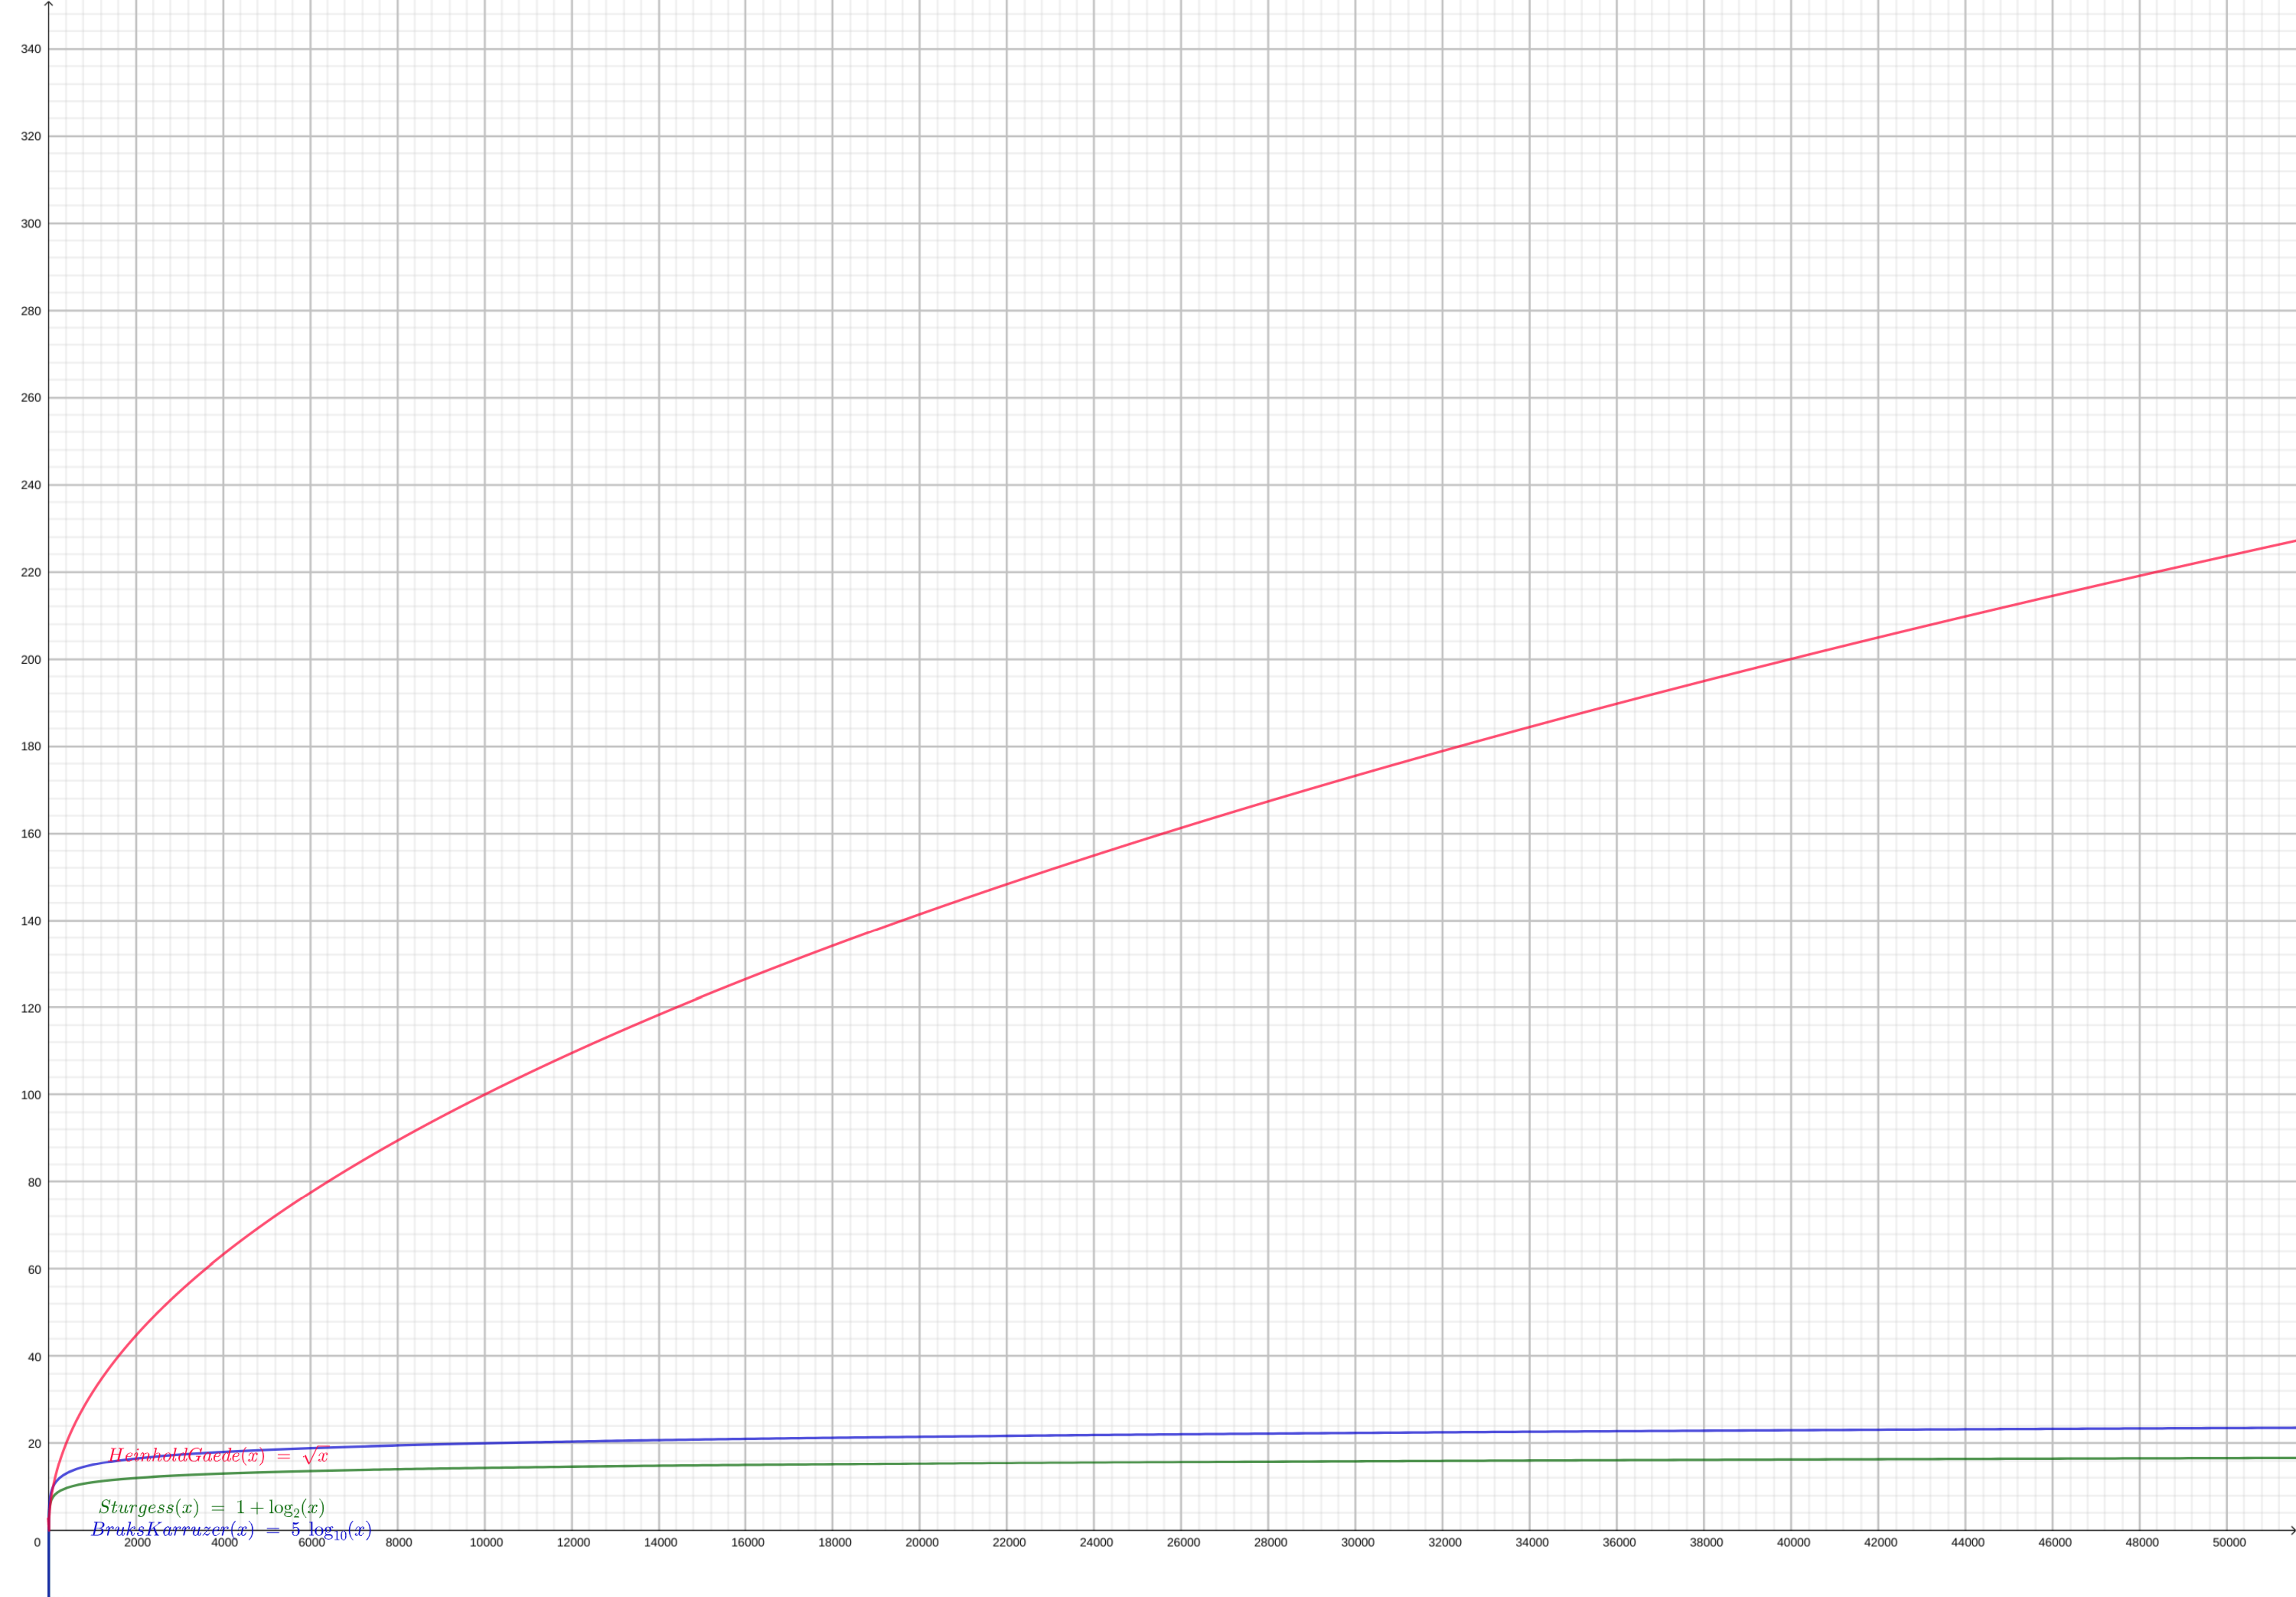
\includegraphics[width=\textwidth]{k-hist-2.pdf}
	\caption{Визуализация числа~k при~$n < 50000$ в~случае использования методов, основанных на~значении $n$}\label{fig:k-hist-n2}
\end{figure}
В~настоящее время наибольшее распространение получила формула Стёрджесса~(формулы \ref{eq:hist_Sturgess-2}, \ref{eq:hist_Sturgess-3}). 
\subparagraph{Методы определения числа $k$ на~основе критерия согласия $\chi^{2}$}\label{k-hist:chi-methods}
\par
Сам~по~себе критерий $\chi ^ {2}$ не~может быть использован без~разбиения выборки на~интервалы, в~которых производится вычисление частных разностей между теоретической моделью и~эмпирической выборкой~\cite{Nowiczkij:oczenka-pogresh}. Исходной предпосылкой эффективности применения критерия $\chi^{2}$ является использование интервалов, имеющих не~равную длину, а~равную вероятность в~соответствии с~теоретической моделью. Следует сказать, что~число $m$ интервалов равной длины и~число $k$ равной вероятности могут существенно отличаться.

В~1942 году Х.~Манном и~А.~Вальдом было установлено, что~при~$n \longrightarrow \infty$ оптимальное число равновероятных интервалов $k$ может быть определено по~формуле
\begin{equation}\label{eq:hist_Mann-Wald}
k \approx 4 \sqrt[5]{2} (\frac{n}{t})^{0.4},
\end{equation}
где $t$ "--- квантиль нормального распределения, соответствующий заданной вероятности
\begin{equation}\label{eq:hist_Mann-Wald1}
P = 1 - p,
\end{equation}
где $p$ "--- принятый уровень значимости~\cite{Mann-Wald:Number-of-Class-Intervals}.

В~1950~году K.~Уильямс в~работе~\cite{Williams:choice-of-k} показал, что~коэффициент $4$ может быть заменён на~$2$ без~существенной потери информации. Таким образом, формула приобретает вид
\begin{equation}\label{eq:hist_Williams}
k \approx 2 \sqrt[5]{2} (\frac{n}{t})^{0.4},
\end{equation}
В~1973~году М.~Кендалом и~А.~Стюартом в~работе~\cite{Stat-vyvody-i-svyazi} было предложено дальнейшее развитие формулы~\ref{eq:hist_Mann-Wald}
\begin{equation}\label{eq:hist_Kendall-Stuart}
k \leq b [\sqrt{2}\frac{(n-1)}{t_{1}+t_{2}}]^{0.4},
\end{equation}
где $2 \leq b \leq 4$ 

$t_1, t_2$ "--- некоторые задаваемые квантили


В~1967~году Г.~Хан и~С.~Шапиро в~работе \cite{Hahn&Shapiro:StatModelEng} предложили упрощённый вариант формулы
\begin{equation}\label{eq:hist_Hahn-Shapiro}
k = 4 [0.75 (n-1)^2]^{0.2},
\end{equation}
что может быть получено при~подстановке в~формулу~\ref{eq:hist_Kendall-Stuart} $b = 4, t = 1.645$. В~случае $b = 2$ выражение принимает вид
\begin{equation}\label{eq:hist_Hahn&Shapiro2}
k = 1.9n^{0.4}
\end{equation}
На~рисунках~\ref{fig:k-hist-n3},~\ref{fig:k-hist-n4} показана зависимость $k$ от~$n$, определяемая на~основе критерия согласия~$\chi ^ 2$.
\begin{figure}[ht]
	\centering % Центрируем картинку
	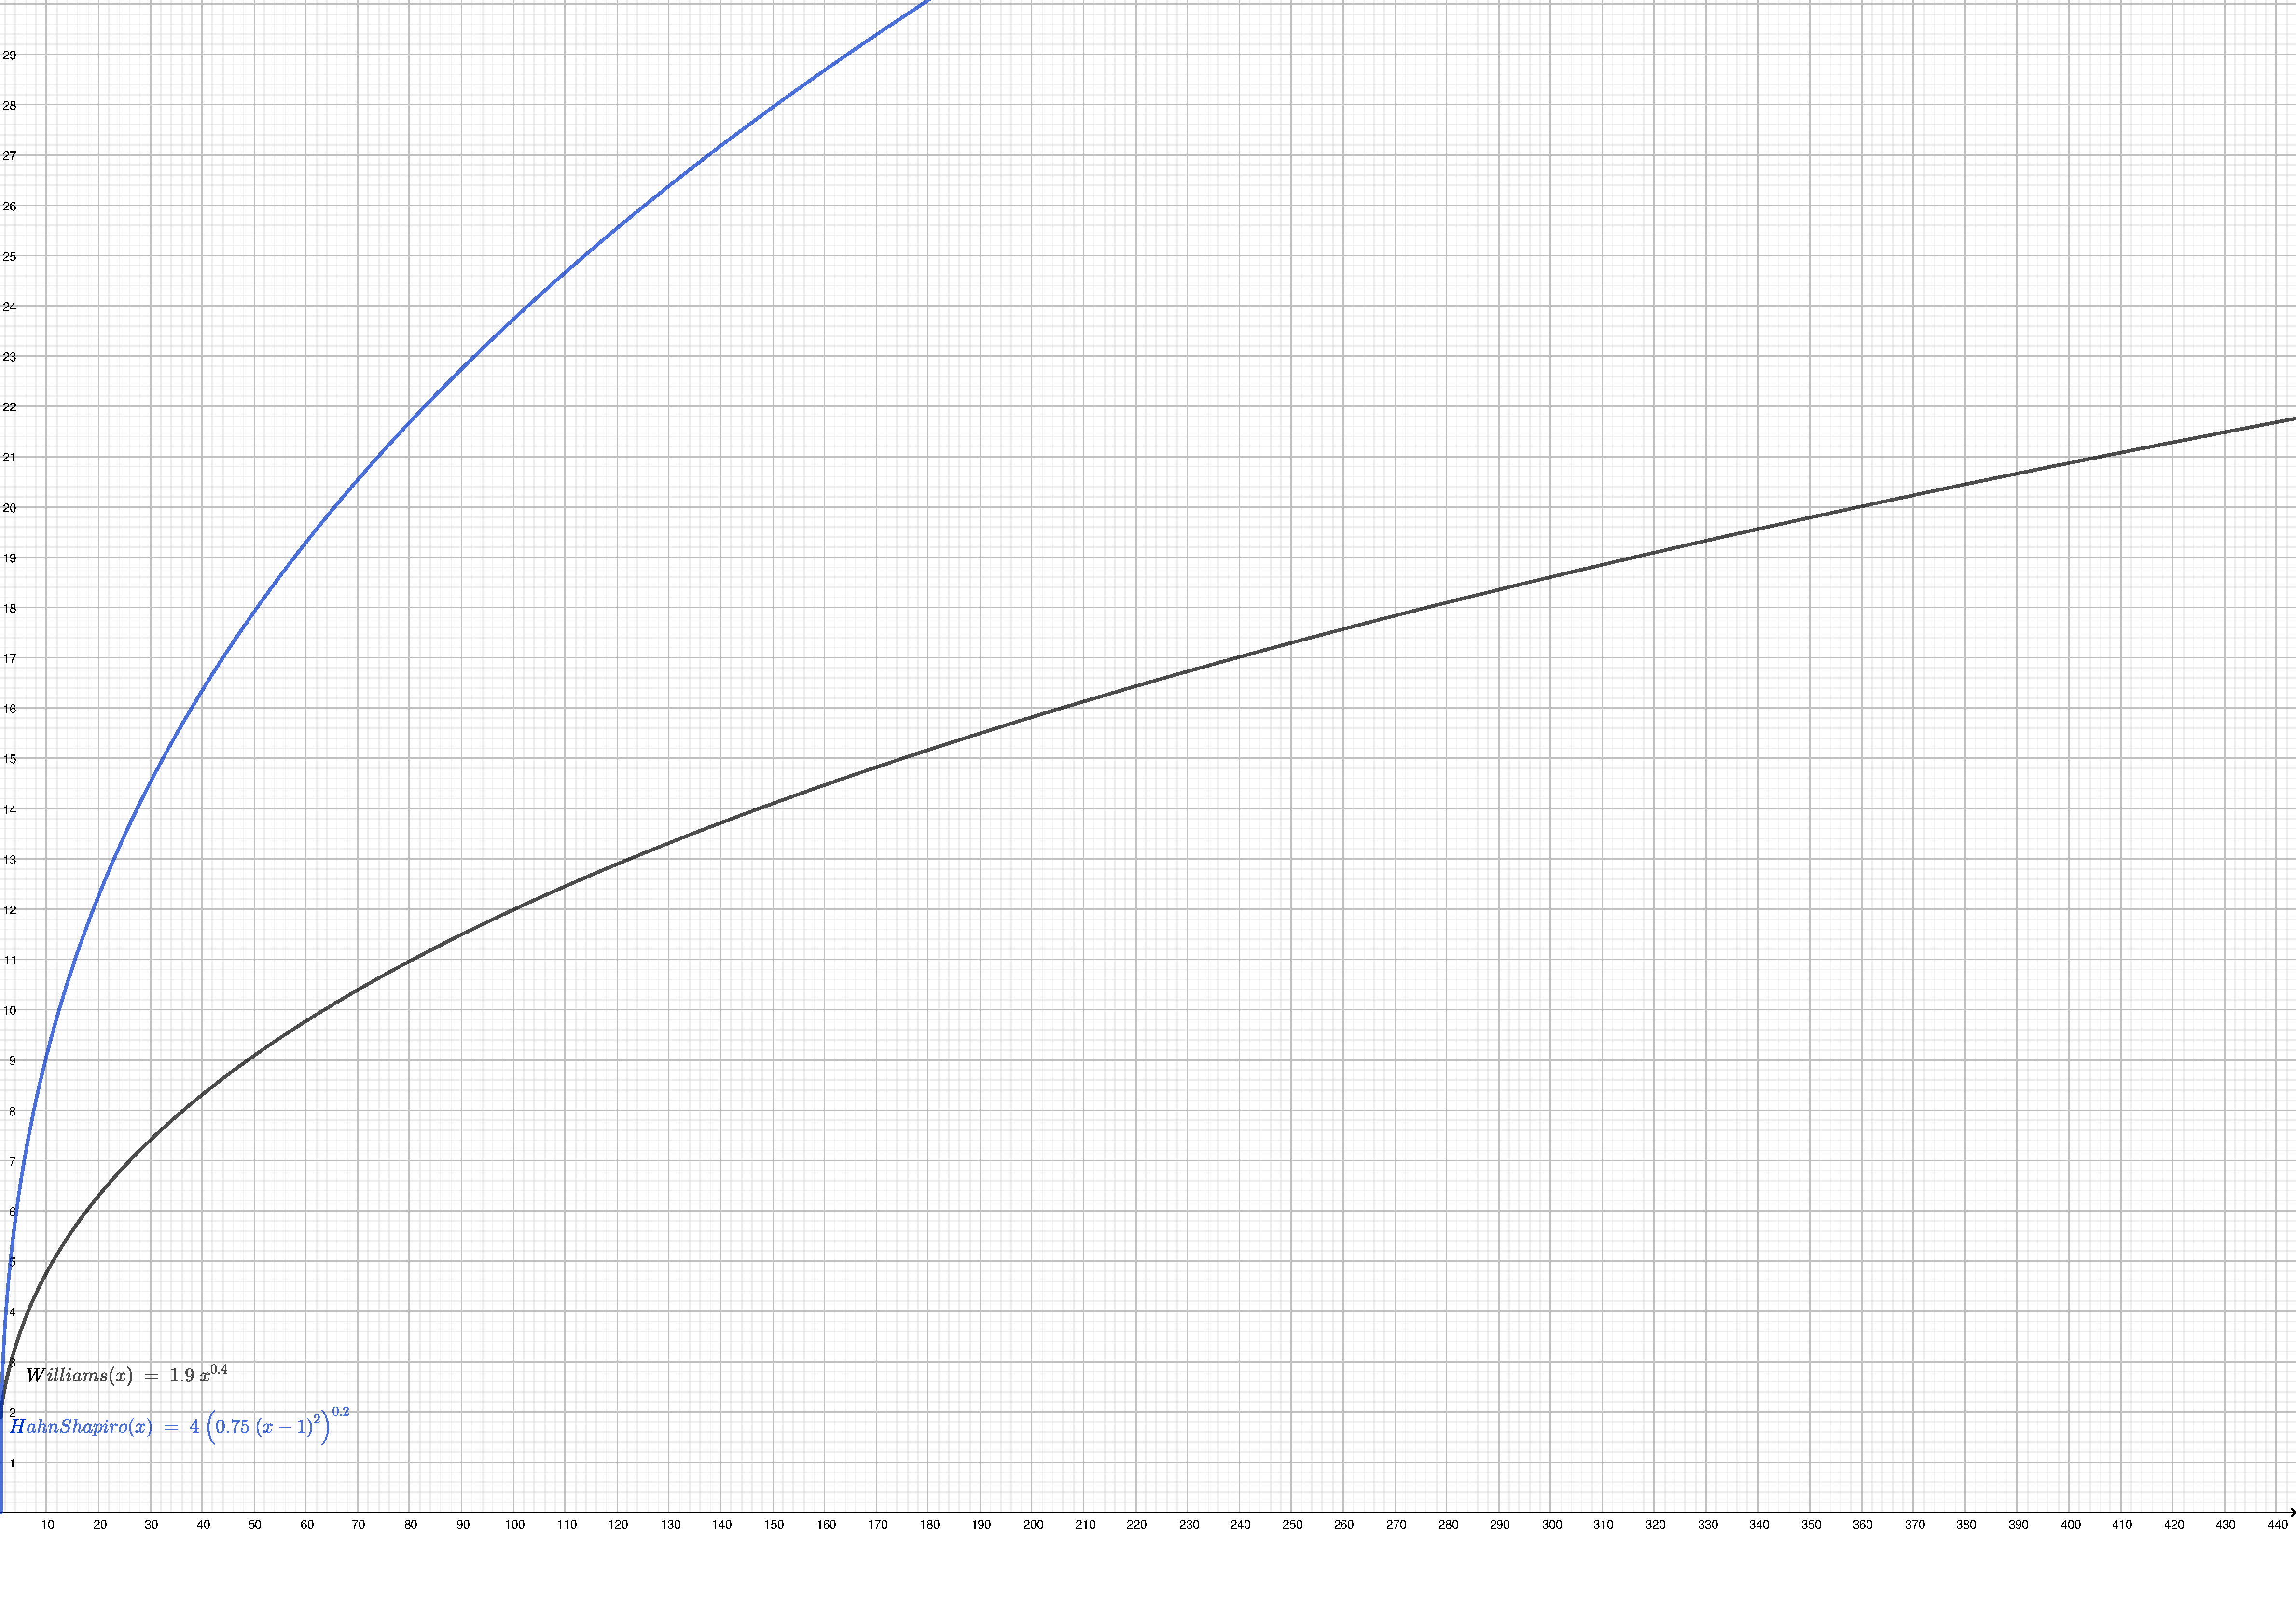
\includegraphics[width=\textwidth]{k-hist-3.pdf}
	\caption{Визуализация числа~k при~$n < 400$ в~случае использования методов, основанных на~критерии согласия $\chi^2$}\label{fig:k-hist-n3}
\end{figure}

\begin{figure}[ht]
	\centering % Центрируем картинку
	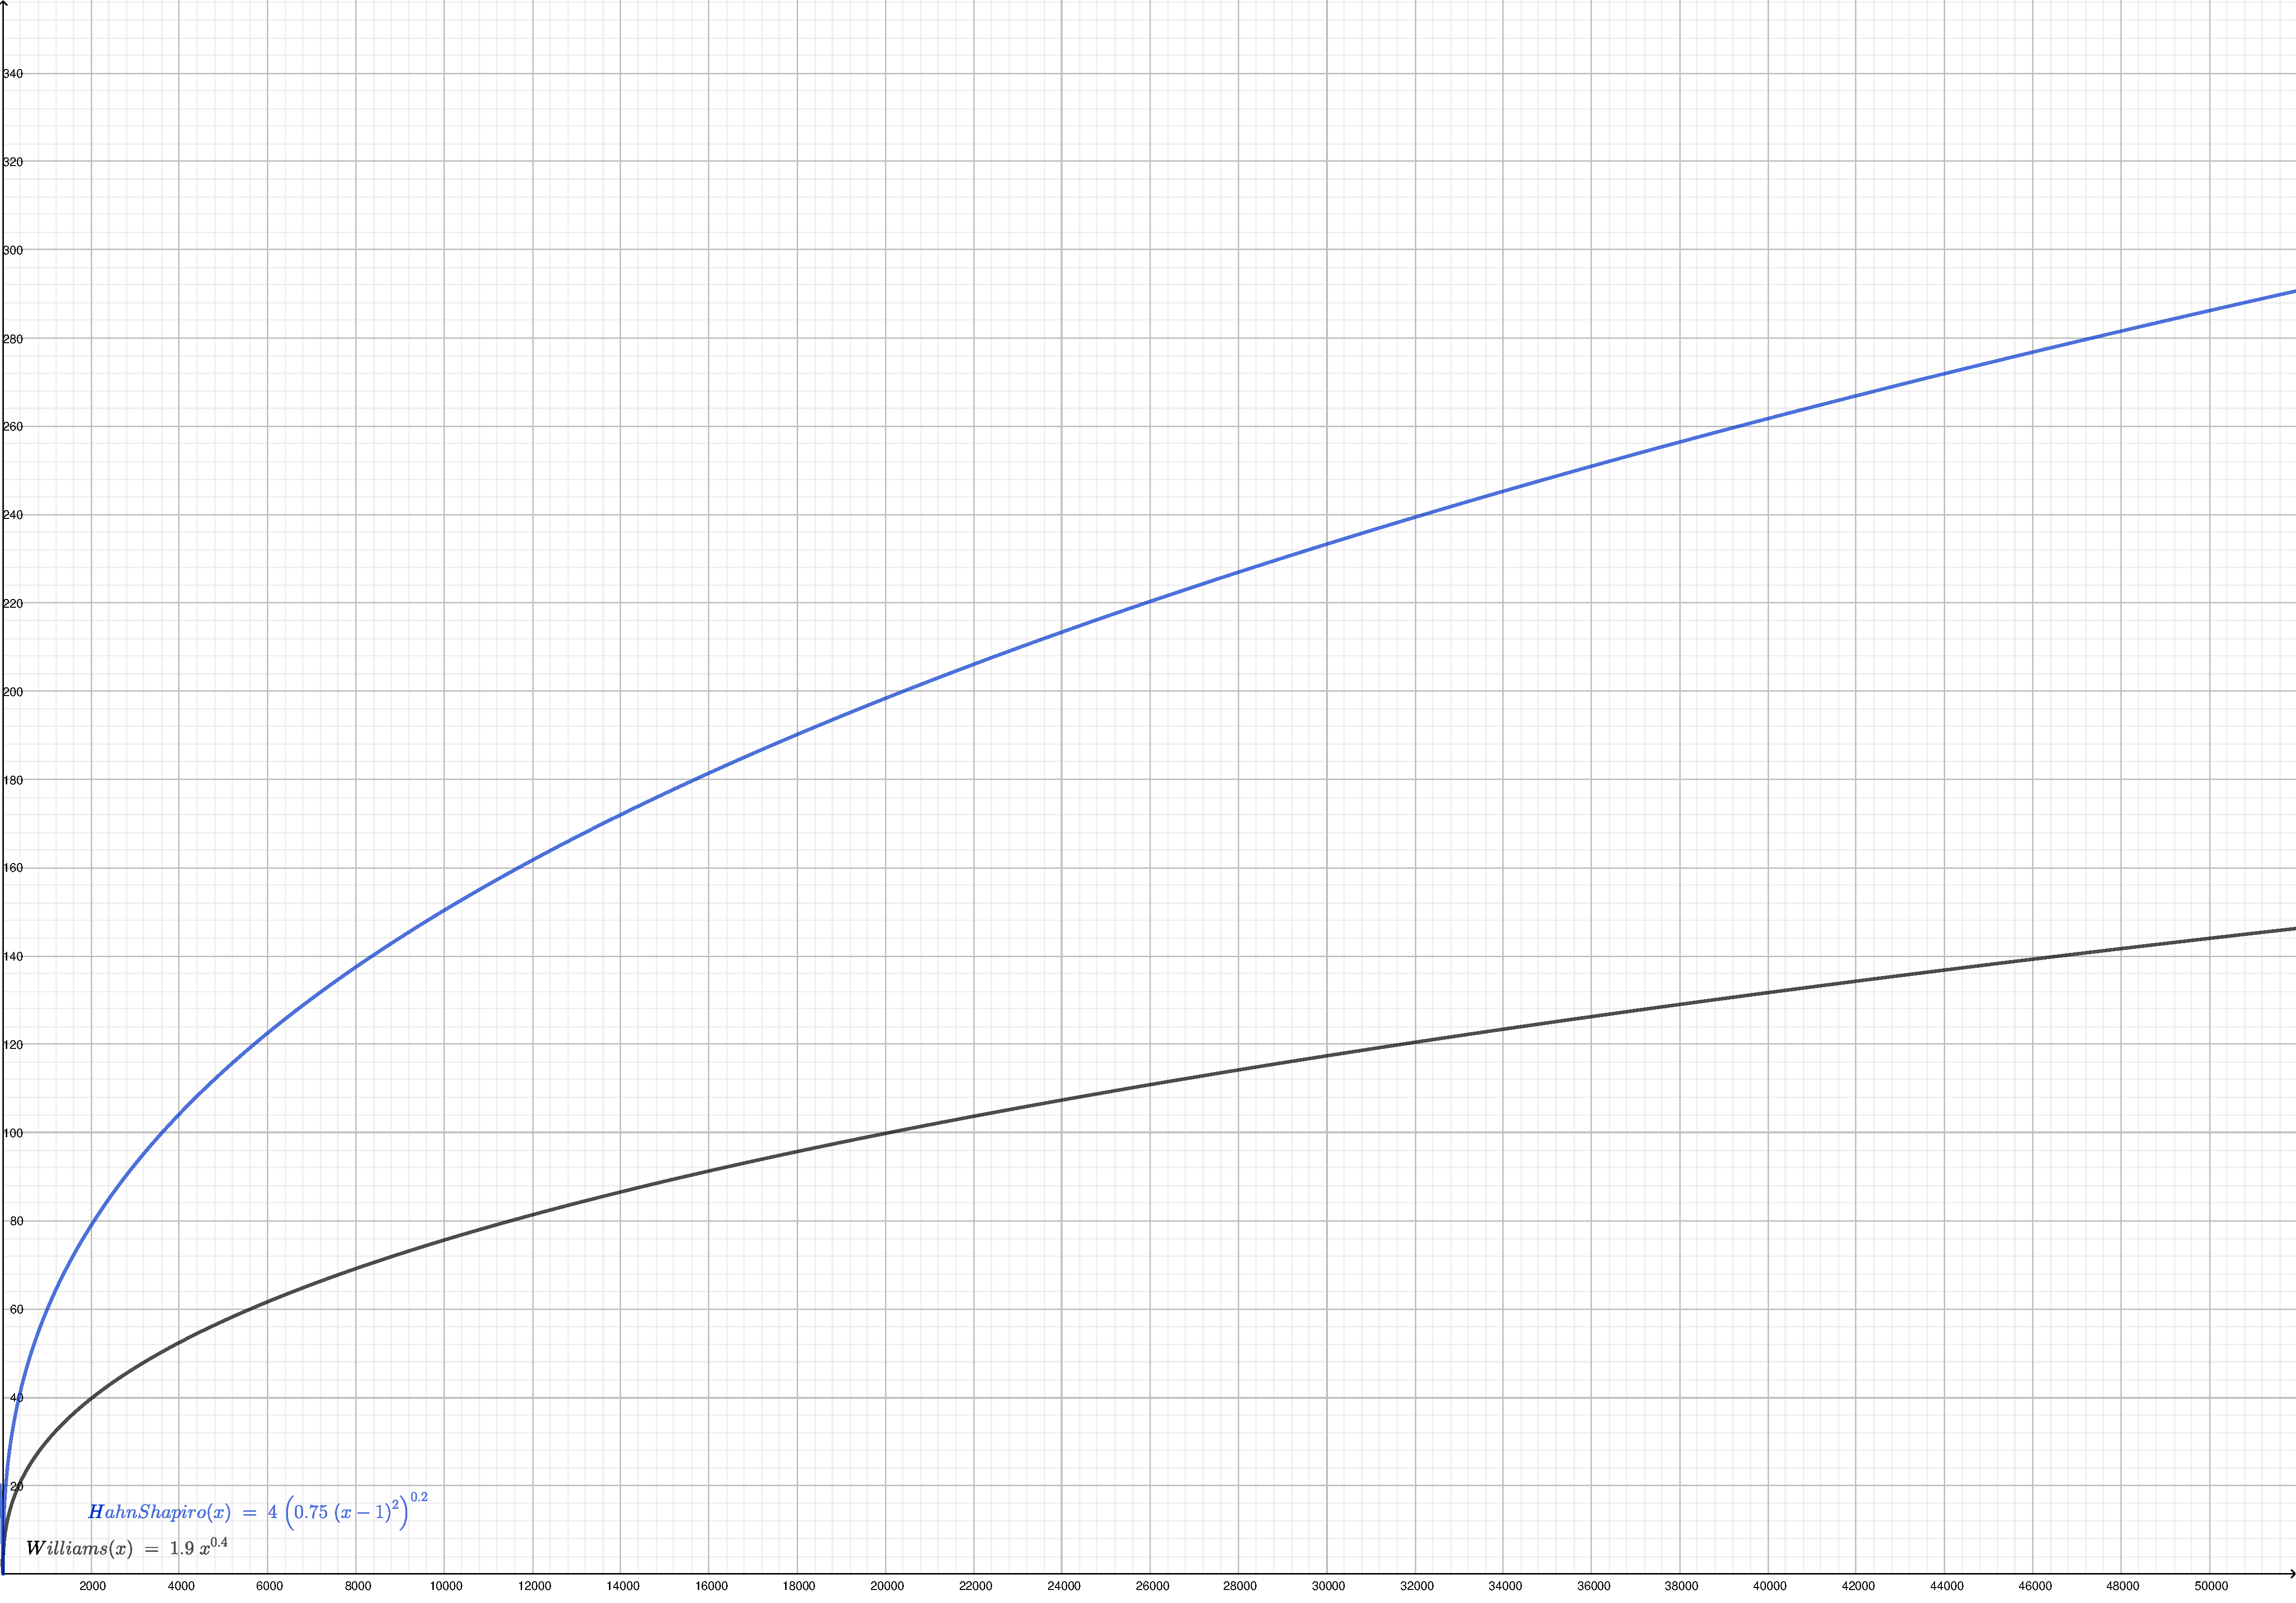
\includegraphics[width=\textwidth]{k-hist-4.pdf}
	\caption{Визуализация числа~k при~$n < 50000$ в~случае использования методов, основанных на~критерии согласия $\chi^2$}\label{fig:k-hist-n4}
\end{figure}
\subparagraph{Методы определения числа $k$ на~основе энтропийного коэффициента}\label{k-hist:entrop-methods}

В~1970--1980-е годы был~проведён ряд исследований, основанных на~использовании критерия близости в~виде энтропийного коэффициента $k_\partial$. Понятий энтропийного коэффициента как~числовой характеристики формы распределения впервые было предложено П.~В.~Новицким в~\cite{Nowiczkij:Entrop-koef}. В~случае c~гистограммой в~соответствии с~\cite{Nowiczkij:Elektrich} эта~оценка вычисляется как
\begin{equation}\label{eq:hist_Nowiczkij}
k_\partial = \frac{dn}{2\sigma}10^{-\frac{1}{n}\sum\limits_{j=1}^n n_j \log_{10}n_j},
\end{equation}
где~$d$ "--- ширина столбца гистограммы,

$\sigma$ "--- стандартное отклонение,

$m$ "--- число столбцов гистограммы,

$n_j$ "--- число наблюдений в~j-ном столбце.

В~результате работ  под~руководством З.\,Таушанова, основанных на~вышеуказанном принципе, в~1973~году в~работе~\cite{Taushanow-k-hist} было выведено соотношение
\begin{equation}\label{eq:hist_Taushanow}
k = 4 \log_{10}{n}
\end{equation}

D~1981 году дальнейшее развитие формулы \ref{eq:hist_Taushanow} со~стороны Е.\,Тоневой~\cite{Tonewa:k-hist} привело к~разработке соотношения
\begin{equation}\label{eq:hist_Tonewa}
k = 5 \lg n - 5 \equiv 5 \lg (\frac{n}{10}).
\end{equation}

На~рисунках \ref{fig:k-hist-n5}, \ref{fig:k-hist-n6} реализована визуализация функции зависимости $k$ от~$n$ в~случае использования методов, основанных на~энтропийном коэффициенте.

\begin{figure}[ht]
	\centering % Центрируем картинку
	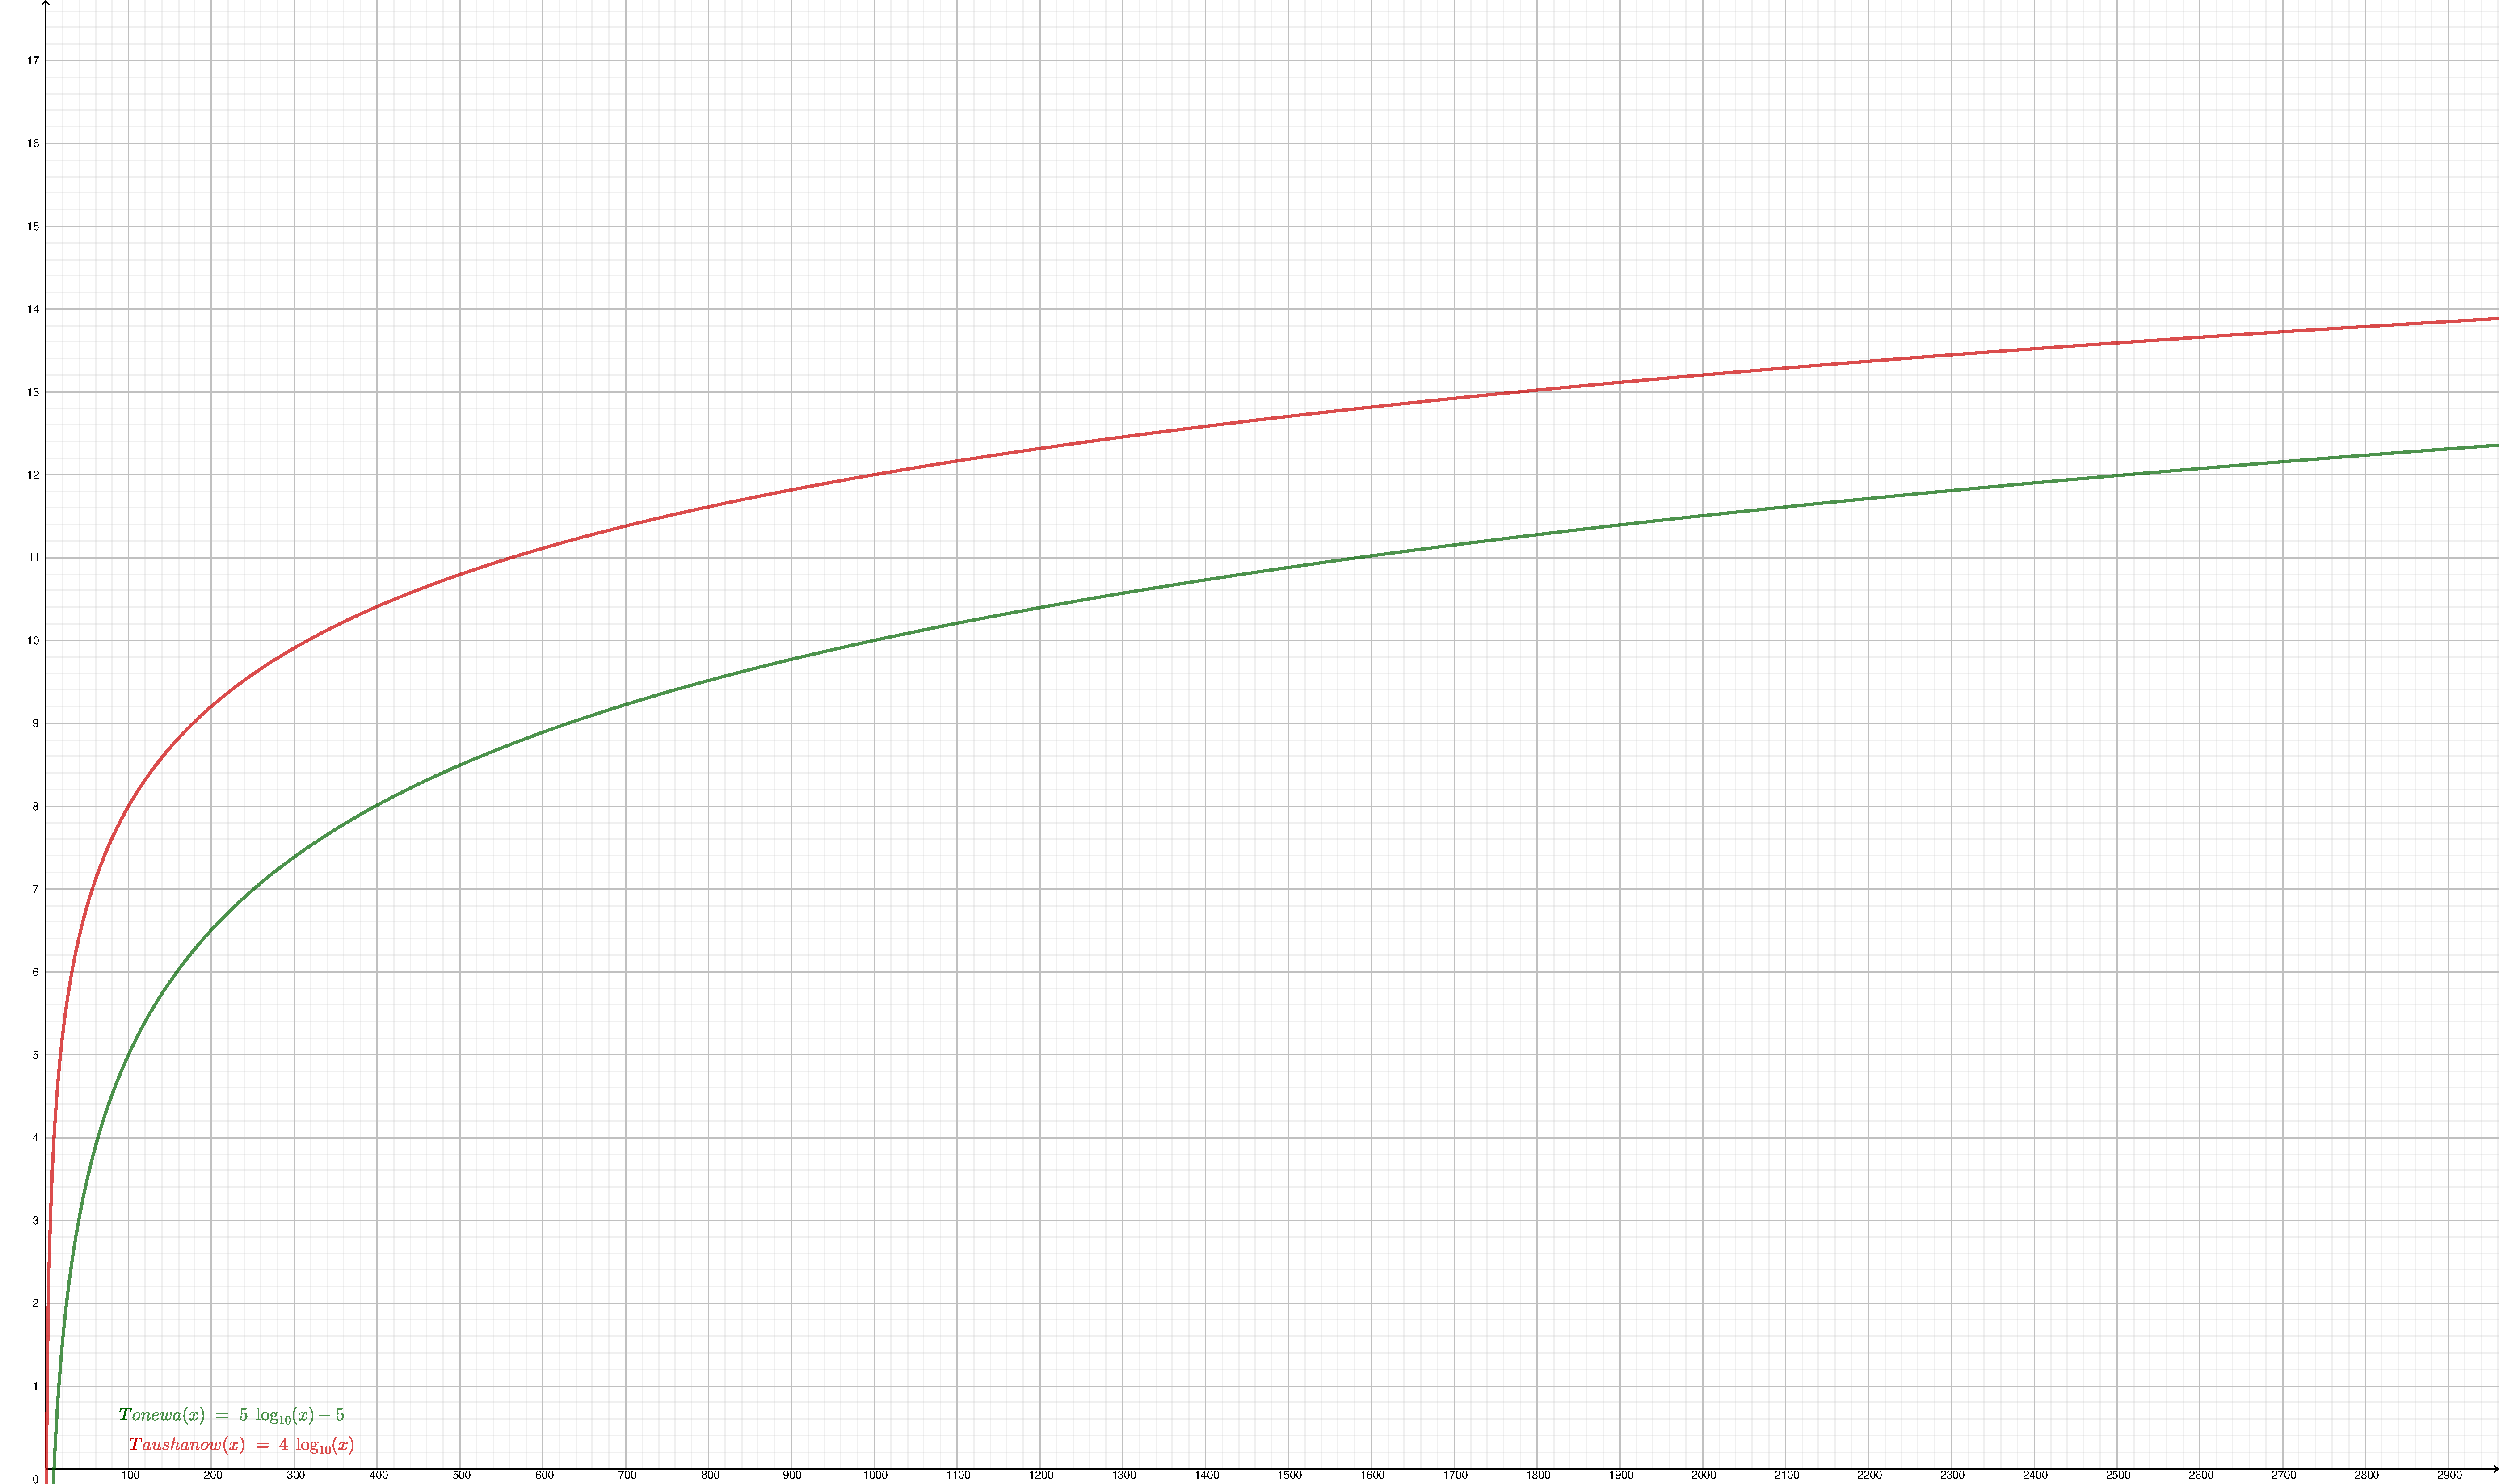
\includegraphics[width=\textwidth]{k-hist-5.pdf}
	\caption{Визуализация числа~$k$ при~$n < 3000$ в~случае использования методов, основанных на~энтропийном коэффициенте}\label{fig:k-hist-n5}
\end{figure}

\begin{figure}[ht]
	\centering % Центрируем картинку
	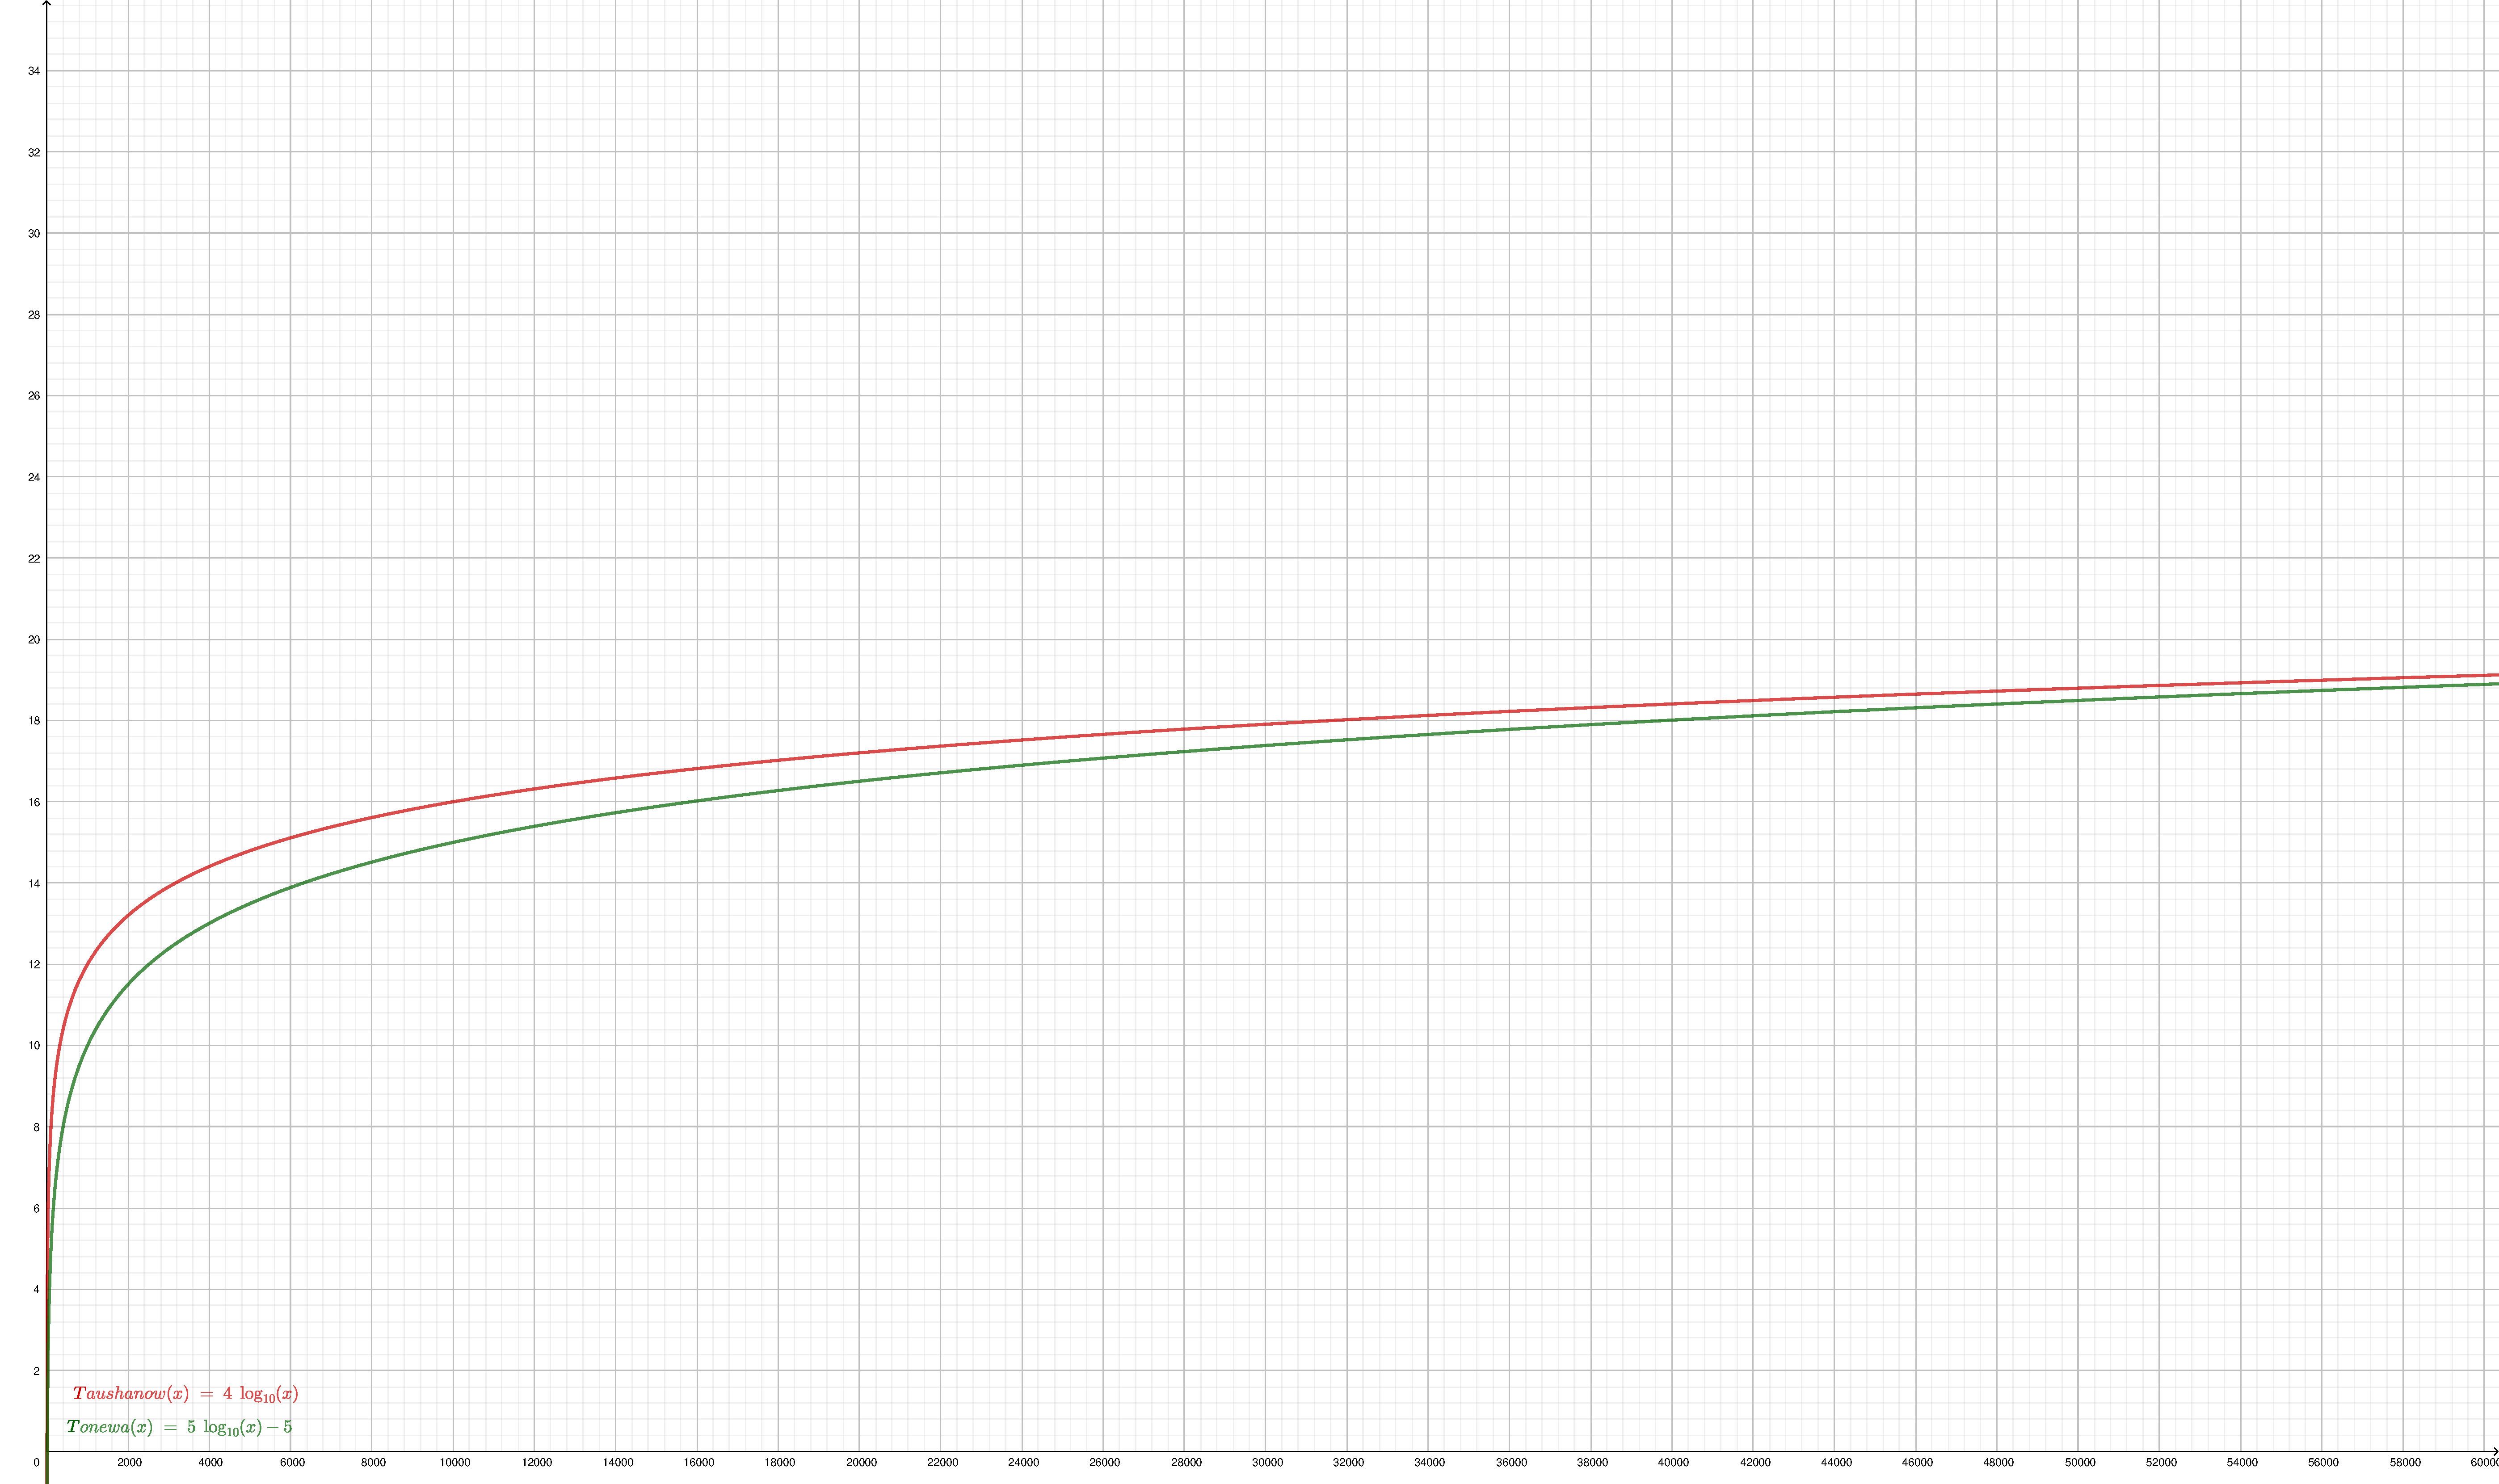
\includegraphics[width=\textwidth]{k-hist-6.pdf}
	\caption{Визуализация числа~$k$ при~$n < 50000$ в~случае использования методов, основанных на~энтропийном коэффициенте}\label{fig:k-hist-n6}
\end{figure}

\subparagraph{Методы определения числа $k$ на~основе четвёртого центрального момента}
\par

Следует отметить, что~все исследования, описанные в~\ref*{k-hist:common-methods}--\ref{k-hist:entrop-methods}, начиная с~работ Стёрджесса, закачивая исследованиями энтропийного коэффициента, рассматривают $k$ исключительно как~функцию~$n$, расходясь только в~выборе вида этой функции.

Принципиально новый подход был~предложен в~1975 году И.~У.~Алексеевой в~работе~\cite{Alekseewa:k-hist}. Согласно выводам, сделанным автором данной работы, $k$ существенно зависит от~значения \emph{коэффициента контрэксцесса}, являющегося величиной обратной \emph{коэффициенту эксцесса}, представляющего в~свою очередь относительную меру \textbf{четвёртого центрального момента}. Вопросы \emph{центральных моментов} рассмотрены в~\ref{moments}. Следует отметить, что~все~центральные моменты взаимосвязаны между собой, таким образом, значение четвёртого содержит в~себе информацию о~первых трёх, что~означает учёт обширной информации о~об~изучаемых данных.
\begin{equation}\label{eq:hist_Alekseewa-0}
k = \frac{4}{\xi}\lg\frac{n}{10},
\end{equation}
где $\xi$ "--- значение контрэксцесса
\begin{equation}\label{eq:kontr-kurtosis}
\xi = \frac{1}{\sqrt{\varepsilon}} == \frac{S^2}{\sqrt{\mu_4}},
\end{equation},
где $\varepsilon$ "--- значение эксцесса,

$S$ "--- дисперсия,

$\mu_4$ "--- четвёртый центральный момент.

Как~было сказано ранее, детальное рассмотрение вопросов центральных моментов проводится в~\ref{moments}.

Формула~\ref{eq:hist_Alekseewa-0} открывает новые возможности анализа при~первичной интерпретации и~визуализации данных. Полученный в~\cite{Alekseewa:k-hist} сдвиг функции $k = f(n)$ может быть аппроксимирован в~зависимости от~значения эксцесса выражениями
\begin{equation}\label{eq:hist_Alekseewa-01}
A(\varepsilon) = \frac{\varepsilon + 1.5}{6}
\end{equation}
либо
\begin{equation}\label{eq:hist_Alekseewa-02}
A(\varepsilon) = \frac{\varepsilon^{0.8}}{3}.
\end{equation}
Вследствие этого дальнейшее развитие формулы~\ref{eq:hist_Alekseewa-0} привело к~разработке соотношений
\begin{equation}\label{eq:hist_Alekseewa-1}
k = \frac{\varepsilon+1.5}{6} n^{0.4},
\end{equation}
а~также
\begin{equation}\label{eq:hist_Alekseewa-2}
k = \frac{1}{3}\sqrt[5]{\varepsilon^4 n^2} \equiv \frac{1}{3} \sqrt[5]{\frac{n^2}{\xi^8}}.
\end{equation}
Далее на~основе формулы~\ref{eq:hist_Alekseewa-0} было выведено правило, согласно которому
\begin{equation}\label{eq:hist-Alekseewa_3}
0.55n^{0.4} \leq k \leq 1.25n^{0.4}
\end{equation}
При~этом рекомендуется выбирать нечётный $k$, поскольку в~противном случае возникает эффект принудительного уплощения центра гистограммы~\cite{Nowiczkij:oczenka-pogresh}.

\subparagraph{Выводы по~итогам анализа методов определения $k$}
На~основе изложенного выше можно сделать следующие выводы:
	\begin{enumerate}
		\item задача выбора числа интервалов группировки данных выборки представляет собой задачу оптимизации отклонений гистограммы от~кривой плотности распределения, соответствующей генеральной совокупности;
		\item существует такое значение $k$, которое является оптимальным с~точки зрения близости полигона гистограммы к~плавной кривой плотности распределения генеральной совокупности при~данном законе распределения и~данном размере выборки;
		\item использование интервалов равной вероятности вместо равно длины позволяет учитывать форму закона распределения (см.~формулу~\ref{eq:hist_Mann&Wald});
		\item в~случае использования интервалов равной длины их~число в~большей степени зависит от~коэффициента эксцесса~$\varepsilon$, а~не~объёма выборки~$n$;
		\item зависимость $k$ от~$n$ лучше всего аппроксимируется выражением $k=A n^{0.4}$, где~$A$ описывается выражениями \ref{eq:hist_Alekseewa-01}, \ref{eq:hist_Alekseewa-02}.
	\end{enumerate}

Далее в~таблице~\ref{tab:k-hist-compr} приводятся сводные данные по~всем методам.

\begin{table}[ht]
	\caption{Обобщение сведений о~методах определения числа интервалов при~построении гистограмм} \label{tab:k-hist-compr}
	\centering% центрируем таблицу
	\begin{tabularx}{\textwidth}{lXcXcc} 
		\hline
		№  & Автор & Год & Формула & Номер & Источник 
		\\ \hline \hline
		\multicolumn{6}{c}{Основанные только на количестве $n$}
		\\ \hline   
		1  & Г.\,Стёрджесс & 1926 & $k = \frac{range}{1 + \log_2 n}$ & \ref{eq:hist_Sturgess-1}  & \cite{Sturgess:hist-intervals}, \cite{Wand:Data-Based-Hist}                                                                \\ \hline
		2  & Г.\,Стёрджесс & 1926 & $k = 1+\log_2 n$ & \ref{eq:hist_Sturgess-2} & \cite{Sturgess:hist-intervals},\cite{Wand:Data-Based-Hist}                              \\ \hline
		3  & Г.\,Стёрджесс & 1926 & $k = 1 + 3.3\lg n$ & \ref{eq:hist_Sturgess-2} & \cite{Sturgess:hist-intervals},\cite{Wand:Data-Based-Hist}                              \\ \hline
		4  &Брукс, Каррузер &?&$k = 5 \lg n$&\ref{eq:hist-Bruks-Karruzer}&\cite{Shtorm:MathStat}
		\\ \hline 
		5  & И\,Хайнхольд, К\,Гаеде & 1965 & $k = \sqrt{n}$ & \ref{eq:hist_Heinholds-Gaede} & \cite{Ingenieur-Statistik}
		\\ \hline
		\multicolumn{6}{c}{Основанные на~критерии согласия~$\chi^2$}
		\\ \hline
		6  & Х.\,Манн, А.\,Вальд & 1942 & $k \approx 4 \sqrt[5]{2} (\frac{n}{t})^{0.4}$ & \ref{eq:hist_Mann-Wald} & \cite{Mann-Wald:Number-of-Class-Intervals}
		\\ \hline
		7  & К.\,Уильямс & 1950 & $k \approx 2 \sqrt[5]{2} (\frac{n}{t})^{0.4}$ & \ref{eq:hist_Williams} & \cite{Williams:choice-of-k}
		\\ \hline
		8  & Г.\,Хан, С\,Шапиро & 1967 & $k = 4 [0.75 (n-1)^2]^{0.2}$ & \ref{eq:hist_Hahn-Shapiro} & \cite{Hahn&Shapiro:StatModelEng}
		\\ \hline
		9 & Г.\,Хан, С\,Шапиро & 1967 & $k = 1.9n^{0.4}$ & \ref{eq:hist_Hahn-Shapiro} & \cite{Hahn&Shapiro:StatModelEng}
		\\ \hline
		10 & М.\,Кендалл, А\,Стюарт & 1970 & $k \leq b [\sqrt{2}\frac{(n-1)}{t_{1}+t_{2}}]^{0.4}$ & \ref{eq:hist_Kendall-Stuart} & \cite{Stat-vyvody-i-svyazi}
		\\ \hline
		\multicolumn{6}{c}{Основанные на~энтропийном коэффициенте}
		\\ \hline
		11 & З.\,Таушанов & 1973 & $k = 4 \log_{10}{n}$ & \ref{eq:hist_Taushanow} & \cite{Taushanow-k-hist}
		\\ \hline
		12 & Е.\,Тонева & 1981 & $k = 5 \lg n - 5 \equiv 5 \lg (\frac{n}{10})$ & \ref{eq:hist_Tonewa} & \cite{Tonewa:k-hist}
		\\ \hline
		\multicolumn{6}{c}{Основанные на~четвёртом центральном моменте}
		\\ \hline
		13 & И\,Алексеева & 1975 & $k = \frac{4}{\xi}\lg\frac{n}{10}$ & \ref{eq:hist_Alekseewa-0} &\cite{Alekseewa:k-hist}
		\\ \hline
		14 & П\,Новицкий & 1991 & $k = \frac{\varepsilon+1.5}{6} n^{0.4}$ & \ref{eq:hist_Alekseewa-1} & \cite{Nowiczkij:oczenka-pogresh}
		\\ \hline
		15 & П\,Новицкий & 1991 & $k = \frac{1}{3}\sqrt[5]{\varepsilon^4 n^2} \equiv \frac{1}{3} \sqrt[5]{\frac{n^2}{\xi^8}}$ & \ref{eq:hist_Alekseewa-2} & \cite{Nowiczkij:oczenka-pogresh}
		\\ \hline
		16 & П\,Новицкий & 1991 & $0.55n^{0.4} \leq k \leq 1.25n^{0.4}$ & \ref{eq:hist-Alekseewa_3} & \cite{Nowiczkij:oczenka-pogresh}
		\\ \hline
		\end{tabularx}
\end{table}

\paragraph{Реализация}
\par
Создадим функции, рассчитывающие число k в~соответствии с~рассмотренными в~\ref{hist-number-of-k} методами. Данное действие не~является обязательным. По~умолчанию R строит гистограммы с~числом $k$, определённым на~основе формулы Стёрджесса (формулы~\ref{eq:hist_Sturgess-3}). Вопросы программирования на~R и~Python рассматриваются в~соответствующих фрагментах. Здесь следует сказать лишь то, можно написать формулу для~конкретного случая и~набора данных, однако хорошей практикой является создание функций, их~сохранение и~многократное использование в~дальнейшей работе. Важно помнить, что~переменные, создаваемые внутри тела функции, не~возникают в~глобальном окружении, вследствие этого им~можно присваивать любые имена. В~скрипте~\ref{lis:optimal-k-R} приведён код, позволяющий определить k всеми 15-ю рассмотренными выше способами. Файл со~скриптом доступен в~репозитории по~\href{https://github.com/Kirill-Murashev/AI_for_valuers_R_source/tree/main/Hist}{ссылке}~\cite{R_source_github}.

\begin{lstlisting}[caption = Создание функций для~автоматизированного определения оптимального значения k, firstnumber=1, language = R, firstnumber=1, numbers=left, numberstyle=\tiny, stepnumber=2, numbersep=5pt, label= lis:optimal-k-R]
kHistSturgess0 <- function(x, na.omit = FALSE){
n   <- NROW(x)
ks0 = (max(x)-min(x))/(1+log2(n)) 
return(c(ks0))                              
}                                               

# создать функцию для первой версии формулы Стёрджесса
kHistSturgess1 <- function(x, na.omit = FALSE){ 
n   <- NROW(x)                              
ks1 = (1+log2(n))                             
return(ks1)                                     
}                                                             

# создать функцию для второй версии формулы Стёрджесса
kHistSturgess2 <- function(x, na.omit = FALSE){ 
n   <- NROW(x)                                
ks2 = (1+(3.3*log10(n)))                     
return(ks2)                                   
}                                             

# создать функцию для формулы Брукса и Каррузера
kHistBruksKarruzer <- function(x, na.omit = FALSE){ 
n   <- NROW(x)                                    
kbk = 5*log10(n)                                  
return(kbk)                                       
}                                                   

# создать функцию для формулы Хайнхольда и Гаеде
kHistHeinholdGaede <- function(x, na.omit = FALSE){ 
n   <- NROW(x)                                    
khg = sqrt(n)                                     
return(khg)                                      
}                                                   

# создать функцию для формулы Манна и Вальда
kHistMannWald <- function(x, na.omit = FALSE){ 
n   <- NROW(x)                               
kmw = (4*(2^(1/5)))*((n/qnorm(0.95))^0.4)   
return(kmw)                                   
}                                             

# создать функцию для формулы Уильямса
kHistWilliams <- function(x, na.omit = FALSE){ 
n   <- NROW(x)                               
kwi = (2*(2^(1/5)))*((n/qnorm(0.95))^0.4)    
return(kwi)                                   
}                                            

# создать функцию для первой формулы Хана и Шапиро
kHistHahnShapiro <- function(x, na.omit = FALSE){ 
n   <- NROW(x)                                 
khs = 4*(0.75*((n-1)^2)^0.2)                   
return(khs)                                   
}                                                 

# создать функцию для второй формулы Хана и Шапиро
kHistShapiroHahn <- function(x, na.omit = FALSE){ 
n   <- NROW(x)                                  
ksh = 1.9*(n^0.4)                              
return(ksh)                                     
}                                                

# создать функцию для формулы Кендалла и Стюарта
kHistKendallStuart <- function(x, na.omit = FALSE){ 
n   <- NROW(x)                                   
b = 2                                            
t1 = qnorm(0.95)                                
t2 = 0                                           
kks = b*(sqrt(2)*(((n-1)/(t1+t2))^0.4))          
return(kks)                                    
}                                                  

# создать функцию для формулы Таушанова
kHistTaushanow <- function(x, na.omit = FALSE){ 
n   <- NROW(x)                                
kta = 4*log10(n)                             
return(kta)                                     
}                                              

# создать функцию для формулы Тоневой
kHistTonewa <- function(x, na.omit = FALSE){ 
n   <- NROW(x)                            
kto = 5*log10(n)-5                         
return(kto)                               
}                                           

# создать функцию для формулы Алексеевой
kHistAlekseewa <- function(x, na.omit = FALSE){
n   <- NROW(x)                               
kurt = kurtosis(x)                          
counterkurt = 1/(sqrt(kurt))                 
kal = (4/counterkurt)*(log10(n/10))         
return(kal)                                 
}                                             

# создать функцию для первой формулы Новицкого
kHistNowiczkij1 <- function(x, na.omit = FALSE){ 
n   <- NROW(x)                                
kurt = kurtosis(x)                             
kn1 = ((kurt+1.5)/6)*(n^0.4)                  
return(kn1)                                   
}                                               

# создать функцию для второй формулы Новицкого
kHistNowiczkij2 <- function(x, na.omit = FALSE){ 
n   <- NROW(x)                                
kurt = kurtosis(x)                             
kn2 = (((kurt^4)*(n^2))^(1/5))*(1/3)           
return(kn2)                                    
}                                               

# создать функцию для третьей формулы Новицкого
kHistNowiczkij3_min <- function(x, na.omit = FALSE){ 
n   <- NROW(x)                                     
kurt = kurtosis(x)                                 
kn3min = 0.55*(n^0.4)                             
return(kn3min)                                    
}                                                   

# создать функцию для третьей формулы Новицкого
kHistNowiczkij3_max <- function(x, na.omit = FALSE){
n   <- NROW(x)                                   
kurt = kurtosis(x)                                
kn3max = 1.25*(n^0.4)                             
return(kn3max)                                    
}                                                   

optimalK <- function(x, na.omit = FALSE){ 
ks0 <- kHistSturgess0(x)
ks1 <- kHistSturgess1(x)
ks2 <- kHistSturgess2(x)
kbk <- kHistBruksKarruzer(x)
khg <- kHistHeinholdGaede(x)
kmw <- kHistMannWald(x)
kwi <- kHistWilliams(x)
khs <- kHistHahnShapiro(x) 
ksh <- kHistShapiroHahn(x)
kks <- kHistKendallStuart(x)
kta <- kHistTaushanow(x)
kto <- kHistTonewa(x)
kal <- kHistAlekseewa(x)
kn1 <- kHistNowiczkij1(x)
kn2 <- kHistNowiczkij2(x)
kn3_min <- kHistNowiczkij3_min(x)
kn3_max <- kHistNowiczkij3_max(x)
optimal_k <- return(c(ks0, ks1, ks2, kbk, khg, kmw, kwi,
	khs, ksh, kks, kta, kto, kal, kn1, kn2, kn3_min, kn3_max))
return(k)
}
\end{lstlisting}

Далее применим функции к~набору данных <<almatyFlats>> (см.~скрипт\ref{lis:optimal-k-almaty}).
\begin{lstlisting}[float, caption = Создание функций для~автоматизированного определения оптимального значения k, firstnumber=1, language = R, firstnumber=1, numbers=left, numberstyle=\tiny, stepnumber=2, numbersep=5pt, label= lis:optimal-k-almaty]
optimal_k <- optimalK(almatyFlats$price.m)  
function_name<- c("Sturgess0",
	 "Sturgess1",
	 "Sturgess2",
	 "BruksKarruzer",
	 "HeinholdGaede",
	 "MannWald",
	 "Williams",
	 "HahnShapiro",
	 "ShapiroHahn",
	 "KendallStuart",
	 "Taushanow",
	 "Tonewa",
	 "Alekseewa",
	 "Nowiczkij1",
	 "Nowiczkij2",
	 "Nowiczkij3_min",
	 "Nowiczkij3_max")
k_optimal <- tibble(function_name, optimal_k)
\end{lstlisting}

 В~результате были получены следующие значения k~(см.~таблицу~\ref{tab:k-hist-optimal-almaty}).
 
 Для~сравнения также был проведён анализ оптимального $k$ для~рынка квартир городской агломерации Санкт-Петербург. Для~этого взят набор данных <<spba\_flats\_210928>>~\cite{ds:spba-flats-210928}, собранный автором 28~сентября~2021 года путём парсинга сайта \href{cian.ru}{cian.ru} и~содержащий сведения о~34821 предложениях. Все~наборы данных, использованные при~составлении данного фрагмента, доступны в~\href{https://github.com/Kirill-Murashev/datasets}{репозитории}~\cite{R_source_github}. Результаты расчётов $k$ приведены в~таблице~\ref{tab:k-hist-optimal-spba}.

\begin{table}[ht]
	\caption{Оптимальное значение $k$ для~переменной, содержащей сведения об~удельной цене предложения на~квартиры в~г.~Алматы, полученное различными методами} \label{tab:k-hist-optimal-almaty}
	\centering% центрируем таблицу
	\begin{tabularx}{\textwidth}{lXX} 
		\hline
		№  & Метод & Значение $k$ 
		\\ \hline \hline
	1 & Sturgess0 & 66513.973 \\ 
	2 & Sturgess1 & 12.202 \\ 
	3 & Sturgess2 & 12.128 \\ 
	4 & BruksKarruzer & 16.860 \\ 
	5 & HeinholdGaede & 48.528 \\ 
	6 & MannWald & 84.064 \\ 
	7 & Williams & 42.032 \\ 
	8 & HahnShapiro & 66.964 \\ 
	9 & ShapiroHahn & 42.418 \\ 
	10 & KendallStuart & 51.739 \\ 
	11 & Taushanow & 13.488 \\ 
	12 & Tonewa & 11.860 \\ 
	13 & Alekseewa & 25.219 \\ 
	14 & Nowiczkij1 & 31.869 \\ 
	15 & Nowiczkij2 & 35.560 \\ 
	16 & Nowiczkij3\_min & 12.279 \\ 
	17 & Nowiczkij3\_max & 27.907 \\
	\hline	
	\end{tabularx}
\end{table}

\begin{table}[ht]
	\caption{Оптимальное значение $k$ для~переменной, содержащей сведения об~удельной цене предложения на~квартиры в~городской агломерации Санкт-Петербург, полученное различными методами} \label{tab:k-hist-optimal-spba}
	\centering% центрируем таблицу
	\begin{tabularx}{\textwidth}{lXX} 
		\hline
		№  & Метод & Значение $k$ 
		\\ \hline \hline
		1 & Sturgess0 & 100989.27 \\ 
		2 & Sturgess1 & 16.09 \\ 
		3 & Sturgess2 & 15.99 \\ 
		4 & BruksKarruzer & 22.71 \\ 
		5 & HeinholdGaede & 186.60 \\ 
		6 & MannWald & 246.92 \\ 
		7 & Williams & 123.46 \\ 
		8 & HahnShapiro & 196.72 \\ 
		9 & ShapiroHahn & 124.59 \\ 
		10 & KendallStuart & 151.99 \\ 
		11 & Taushanow & 18.17 \\ 
		12 & Tonewa & 17.71 \\ 
		13 & Alekseewa & 97.56 \\ 
		14 & Nowiczkij1 & 534.62 \\ 
		15 & Nowiczkij2 & 479.03 \\ 
		16 & Nowiczkij3\_min & 36.07 \\ 
		17 & Nowiczkij3\_max & 81.97 \\
		\hline	
	\end{tabularx}
\end{table}

Далее выставим число интервалов по~умолчанию и~построим гистограмму для~рынка Алматы, см.~рисунок~\ref{fig:hist-almaty-1}.

\begin{figure}[ht]
	\centering % Центрируем картинку
	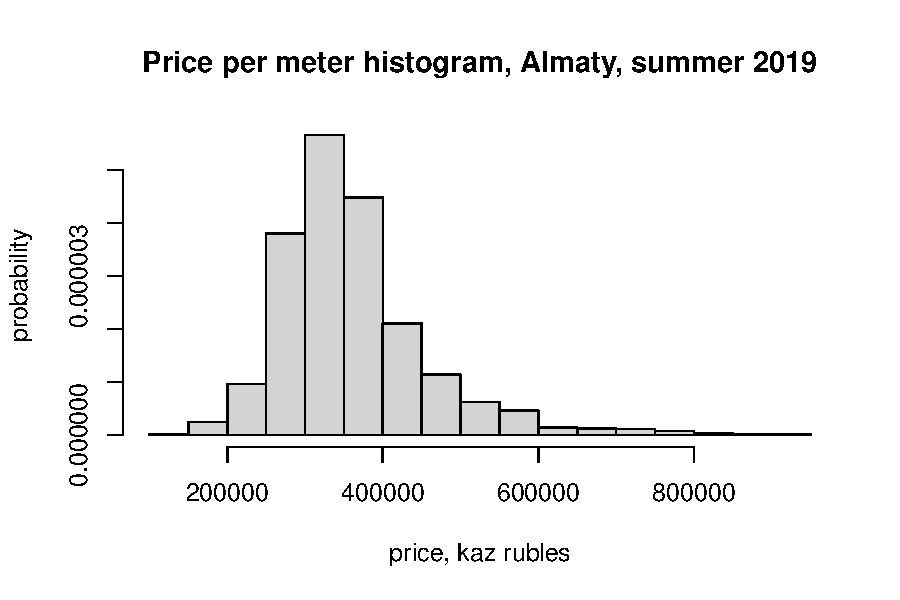
\includegraphics[width=\textwidth]{hist-almaty-1.pdf}
	\caption{Гистограмма удельных цен на~рынке города Алматы (лето 2019~г.)}\label{fig:hist-almaty-1}
\end{figure}

Затем применим формулу~\ref{eq:hist_Alekseewa-01} для~определения числа $k$ и~добавим на~график кривые плотности теоретического нормального и~эмпирического распределений, см.~рисунок~\ref{fig:hist-almaty-2}.

\begin{figure}[ht]
	\centering % Центрируем картинку
	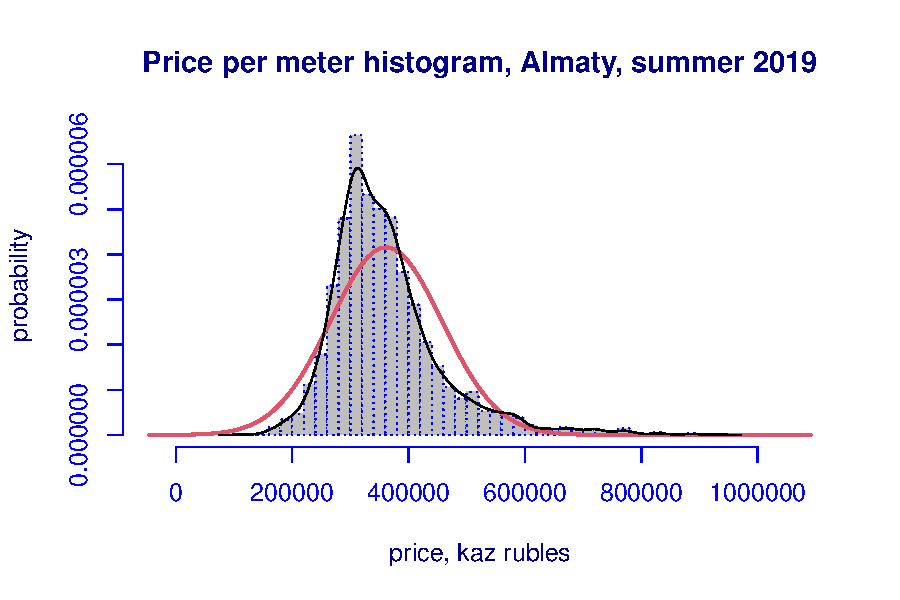
\includegraphics[width=\textwidth]{hist-almaty-2.pdf}
	\caption{Гистограмма удельных цен на~рынке города Алматы (лето 2019~г.), совмещённая с~кривыми плотности теоретического нормального и~эмпирического распределений}\label{fig:hist-almaty-2}
\end{figure}

Для~сравнения построим гистограмму для~аналогичной переменной набора данных \cite{ds:spba-flats-210928}, см.~рисунок~\ref{fig:hist-spba-flats-1}.

\begin{figure}[ht]
	\centering % Центрируем картинку
	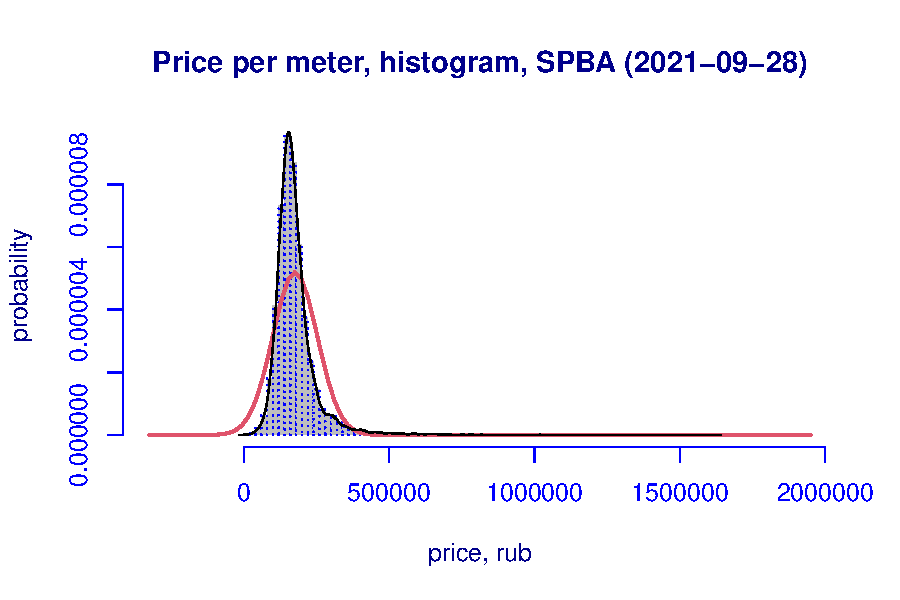
\includegraphics[width=\textwidth]{hist-spba-flats-1.pdf}
	\caption{Гистограмма удельных цен на~рынке города Алматы (лето 2019~г.), совмещённая с~кривыми плотности теоретического нормального и~эмпирического распределений}\label{fig:hist-spba-flats-1}
\end{figure}
Подытоживая вышесказанное, следует повторить, что~в~первую очередь надо смотреть на~площади столбцов, поскольку они~содержат информацию о~вероятности. Во~вторую очередь гистограмма может показать выбросы, что~хорошо видно на~рисунке~\ref{fig:hist-spba-flats-1}.
Скрипты для~построения приведённых гистограмм приведены в~листингах~\ref{lis:hist-almaty-1}, \ref{lis:hist-almaty-2}, \ref{lis:hist-spba-flats-1}.  

\begin{lstlisting}[float, caption = Построение простой гистограммы для~г.~Алматы, firstnumber=1, language = R, firstnumber=1, numbers=left, numberstyle=\tiny, stepnumber=2, numbersep=5pt, label= lis:hist-almaty-1]
hist(almatyFlats$price.m,
	freq = FALSE,
	xlab = "price, kaz rubles",
	ylab = "probability",
	main = "Price per meter histogram, Almaty, summer 2019")
\end{lstlisting}

\begin{lstlisting}[float, caption = Построение гистограммы\, совмещённой с~кривыми плотности теоретического нормального и~эмпирического распределений для~г.~Алматы, firstnumber=1, language = R, firstnumber=1, numbers=left, numberstyle=\tiny, stepnumber=2, numbersep=5pt, label= lis:hist-almaty-2]
histDist(almatyFlats$price.m,
 	nbins = kHistNowiczkij1(almatyFlats$price.m),
	xlab = "price, kaz rubles",
	ylab = "probability",
	main = "Price per meter histogram, Almaty, summer 2019")
lines(density(almatyFlats$price.m))
\end{lstlisting}

\begin{lstlisting}[float, caption = Построение гистограммы\, совмещённой с~кривыми плотности теоретического нормального и~эмпирического распределений для~городской агломерации Санкт-Петербург, firstnumber=1, language = R, firstnumber=1, numbers=left, numberstyle=\tiny, stepnumber=2, numbersep=5pt, label= lis:hist-spba-flats-1]
histDist(spbaFlats$price_m,
	nbins = kHistAlekseewa(spbaFlats$price_m),
	xlab = "price, rub",
	ylab = "probability",
	main = "Price per meter, histogram, SPBA (2021-09-28)")  
lines(density(spbaFlats$price_m))
\end{lstlisting}


\subsubsection{Ядерная оценка плотности}


\subsection{Меры центральной тенденции}

\subsection{Меры изменчивости}

\subsection{Квантили распределения}

\section{Центральные моменты}\label{moments}

\section{Распределения}

\subsection{Нормальное распределение}

\subsection{Логарифмически нормальное распределение}

\subsection{Равномерное распределение}

\subsection{Экспоненциальное распределение}

\subsection{Нормальное распределение}

\subsection{Распределение Вейбулла}

\subsection{Нормальное распределение}

\subsection{Гамма распределение}

\subsection{Бета распределение}

\subsection{Распределение $\chi^{2}$~(Распределение Пирсона)}

\subsection{Распределение Стьюдента~(t-распределение)}

\subsection{Распределение Фишера~(F-распределение)}
 
\subsection{Логистическое распределение}

\subsection{Распределение Парето}

\section{Проверка распределения на~нормальность}

\section{Центральная предельная теорема}

\section{Доверительные интервалы}

\section{Сравнение средних (t-критерий Стьюдента)}

\section{Однофакторный дисперсионный анализ}

\section{ANOVA}

\section{A/B тесты}

\section{Корреляционный анализ}

\subsection{Параметрические методы}

\subsection{Непараметрические методы}

\section{Регрессионный анализ}

\subsection{GLM}

\subsection{Однофакторная линейная регрессия}

\subsection{Множественная регрессия}

\subsection{Логистическая регрессия}

\subsection{Непараметрическая регрессия}







\section{Что~дальше?}
Математическая статистика представляет собой огромную область знаний человека. К~тому~же она~продолжает развиваться. В~данном фрагменте был рассмотрен лишь весьма ограниченный круг вопросов. В~списке источников информации дана некоторая подборка материалов, которые, по~мнению автора, могут быть полезными в~дальнейшем освоении вопросов математической статистики. Поскольку оценщики, как~правило, очень занятые люди, освоение вряд~ли можно ожидать, что~кто-то захочет сразу изучать десятки материалов. В~связи с~этим автор рекомендует ознакомление в~первую очередь со~следующими работами:
	\begin{itemize}
		\item В.\,Cавельев. \emph{Статистика и~котики} ~\cite{Statistika-i-kotiki}. Прекрасная книга для~тех, кто~только начинает погружение в~область математической статистики.
		\item С.\,Бослаф. \emph{Статистика для~всех}~\cite{Statistika-dlya-vsex}. Одна из~лучших книг по~статистике для~тех, кто~не учился по~профилю и~хочет освоить её~методы на~уровне, достаточном для~применения в~профессиональной деятельности.
		\item А.\,Кобзарь. \emph{Прикладная математическая статистика}~\cite{Kobzarq-prikl-mathstat}. Данный материал представляет собой обширное пособие, предназначенное для~тех, кто~уже владеет некоторой базой и~хочет внедрить применение методов математической статистики на~профессиональном уровне.     
	\end{itemize}  

Учиться следует всю~жизнь. Оценочная деятельность трансформируется, и, спустя несколько лет, данное пособие будет казаться детской раскраской. Автор желает читателям непрерывного совершенствования и~становления в~качестве настоящих специалистов в~сфере цифровой оценки XXI~века.

\nocite{Statistika-i-kotiki, Xalqman:Regression-analiz, Baraz:KRA, GOST:Tochnostq-izmerenij-1, GOST:Statmetody, GOST:Statterminy, Stepik:osnovy-statistiki-1, Stepik:osnovy-statistiki-2, Stepik:osnovy-statistiki-3, Teorver-v-uduvolqstvie, CSC:la, CSC:teoriya-grafov, CSC:mathstat-1, CSC:diskt-math, CSC:matan-1, CSC:matan-2, CSC:teorver, CSC:vvedenie-v-matan, Statostika-dlya-gum, Stat-radiosignal, Sprav:mathstat, Math-mod-Kazanczeva, Statistika-dlya-vsex, Veroyatnosty-i-mathstat-Encz, Kobzarq-prikl-mathstat, N-hist, Stat-vyvody-i-svyazi, ITMO:statistika, Drejper-Smith:prikl-regr-analiz, Ajwazyan-prikl-stat, Shixalyyow-Regr-an-par-regr, Biznes-analiz-informaczii:statmetody}

\printbibliography[title=Источники информации]

\end{document}
